% State Of The Art

\chapter{Implementation} % Chapter title

\label{ch:implementation}

%----------------------------------------------------------------------

\section{Statistical variable analysis}
\label{sec:stat-var-analysis}

This section describes the basic properties of each feature we are
using in this particular thesis. Among them we have the count of all
variables, mean, standard deviation, min value, max value, quartiles.
We also add the histogram to have an idea of how the distribution of
the variable works and the boxplot that can help us determine if there
are outliers in the data-set.

\subsection{Average Block Size}
\label{sec:avg-block-size}

A concise definition of a block can be found
\href{https://en.bitcoin.it/wiki/Block}{here}: \textit{``Each block
  contains, among other things, a record of some or all recent
  transactions, and a reference to the block that came immediately
  before it. It also contains an answer to a difficult-to-solve
  mathematical puzzle - the answer to which is unique to each
  block.''}

It's clear that, over time, the size of the block is going to
increase, because there are more and more transactions in the Bitcoin
distributed network, due to that
\autoref{fig:avg-block-size-over-time} shows a non-stoppable
increasing.

This variable, called avg-block-size represent the average size of the
blocks in one day measured in MB. One real number data point each day,
at 18:15:05, spanning from 03/01/2009 to 03/05/2016. It was obtained
from the section \textbf{Charts} of
\href{blockchain.info}{blockchain.info}

\begin{figure}[bth]
  \myfloatalign
  {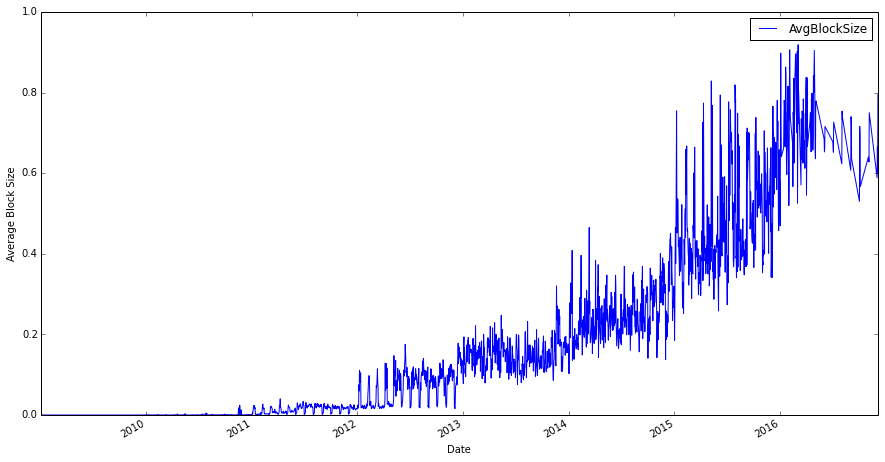
\includegraphics[width=1\linewidth]
    {gfx/avg-block-size-over-time}} 
  \caption{Average Block Size Over Time}
  \label{fig:avg-block-size-over-time}
\end{figure}

In \autoref{fig:avg-block-size-over-time} can be seen how the average
block size has been increasing since the creation of Bitcoin. In 2015
the average block started to dangerously approach the limit of 1 MB,
which is causing a big debate in the Bitcoin community whether they
should increase this limit or not.

\begin{figure}[bth]
  \myfloatalign
  {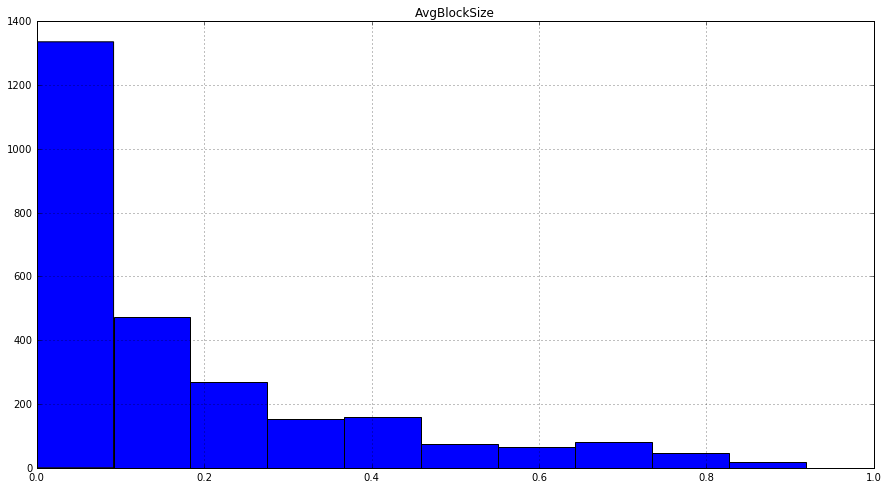
\includegraphics[width=1\linewidth]
    {gfx/avg-block-size-histogram}} 
  \caption{Average Block Size Histogram}
  \label{fig:avg-block-size-histogram}
\end{figure}

\begin{table}
  \myfloatalign
  \small
  \begin{tabularx}{\textwidth}{XX} 
    \toprule
    \tableheadline{Measure} & \tableheadline{Value} \\
    \midrule 
    count  & $2678$\\
    mean   & $0.165078$\\
    median & $0.092355$\\
    std    & $0.209430$\\
    min    & $0.000000$\\
    $25$\% & $0.000899$\\
    $50$\% & $0.092356$\\
    $75$\% & $0.242478$\\
    max    & $0.918519$\\
    \bottomrule
  \end{tabularx}
  \caption{Statistical values for 
    \textit{Average Block Size}}
  \label{tab:stats-avg-block-size}
\end{table}

\begin{figure}[bth]
  \myfloatalign
    {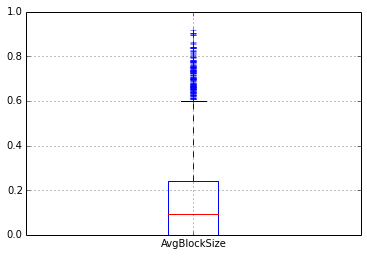
\includegraphics[width=1\linewidth]
      {gfx/avg-block-size-boxplot}}               
    \caption{Average Block Size Boxplot}
    \label{fig:avg-block-size-boxplot}
\end{figure}

\clearpage

%----------------------------------------------------------------------

\subsection{Bitcoin Days Destroyed}
\label{sec:bitcoin-days-destroyed}

\begin{figure}[bth]
  \myfloatalign
  {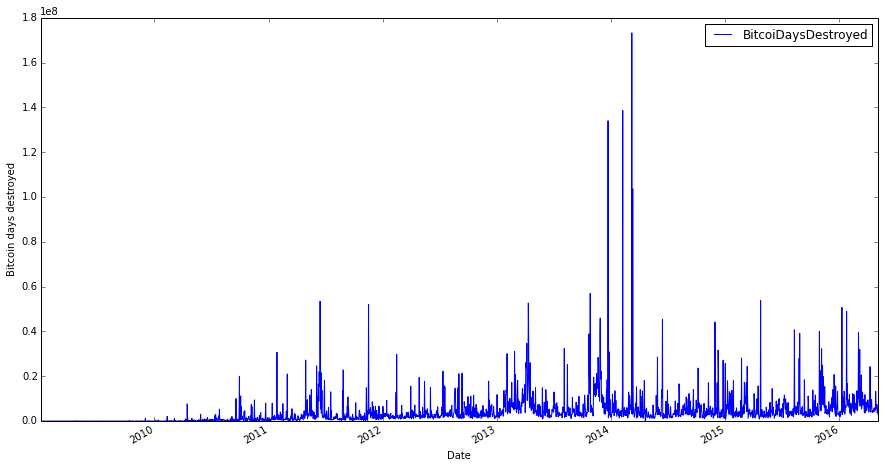
\includegraphics[width=1\linewidth]
    {gfx/bitcoin-days-destroyed-over-time}}
  \caption{Bitcoin Days Destroyed Over Time}
  \label{fig:bitcoin-days-destroyed-over-time}
\end{figure}

Bitcoin Days Destroyed is a weighted measure of aggregate economic
activity, placing value on transacted coins in proportion to the time
they have spent idle on the Bitcoin blockchain. For any given
transaction, Days Destroyed is calculated by multiplying its estimated
transaction value by the number of days since the coins within the
transaction were last spent. Bitcoin Days Destroyed is a useful proxy
for measuring growth in real value transacted on the Bitcoin
blockchain over time, since it controls for rapid movement of coins
between wallets (potentially owned by just one entity). One integer
data point each day, at 18:15:05, spanning from 03/01/2009 to
03/05/2016.

To better understand this variable we include a quote extracted from
\href{http://bitcoin.stackexchange.com/questions/845/what-are-bitcoin-days-destroyed}{Bitcoin
  Beta | Stack Exchange}:

``\textit{The idea of "bitcoin days destroyed" came about because it
  was realized that total transaction volume per day might be an
  inappropriate measure of the level of economic activity in Bitcoin.
  After all, someone could be sending the same money back and forth
  between their own addresses repeatedly. If you sent the same 50 btc
  back and forth 20 times, it would look like 1000 btc worth of
  activity, while in fact it represents almost nothing in terms of
  real transaction volume.}

\textit{With "bitcoin days destroyed", the idea is instead to give
  more weight to coins which haven't been spent in a while. To do
  this, you multiply the amount of each transaction by the number of
  days since those coins were last spent. So, 1 bitcoin that hasn't
  been spent in 100 days (1 bitcoin * 100 days) counts as much as 100
  bitcoins that were just spent yesterday (100 bitcoins * 1 day).
  Because you can think of these "bitcoin days" as building up over
  time until a transaction actually occurs, the actual measure is
  called "bitcoin days destroyed". This is believed to give a better
  indication of how much real economic activity is occurring on the
  bitcoin network.}

\textit{ So how well does it work? Well, it's still not perfect,
  because the other day I moved some coins out of a wallet they've
  been in for several months without spending them or giving them
  away. And some genuine businesses have very rapid turnover in
  bitcoins, so they're not being measured well by this method. But it
  does do a good job of filtering out the "noise" of bitcoins that are
  just "bouncing around" without really going anywhere. The graph of
  overall bitcoin days destroyed is believed to show that the genuine
  level of activity in the Bitcoin economy is continually
  increasing--it's not just one person experimenting by rapidly
  sending the same coins back and forth, flooding the network with
  meaningless chatter. Looks pretty good, hey?}''

\begin{table}
  \myfloatalign
  %\small
  \begin{tabularx}{\textwidth}{XX} 
    \toprule
    \tableheadline{Measure} & \tableheadline{Value} \\
    \midrule 
    count  & $2.679000e+03$ \\
    mean   & $4.146916e+06$ \\
    median & $2456794.0$ \\
    std    & $7.778546e+06$ \\
    min    & $0.000000e+00$ \\
    25\%   & $5.017520e+05$ \\
    50\%   & $2.456794e+06$ \\
    75\%   & $4.745530e+06$ \\
    max    & $1.732980e+08$ \\
    \bottomrule
  \end{tabularx}
  \caption{Statistical values for \textit{Bitcoin Days Destroyed}}
  \label{tab:bitcoin-days-destroyed}
\end{table}

\begin{figure}[bth]
  \myfloatalign
  {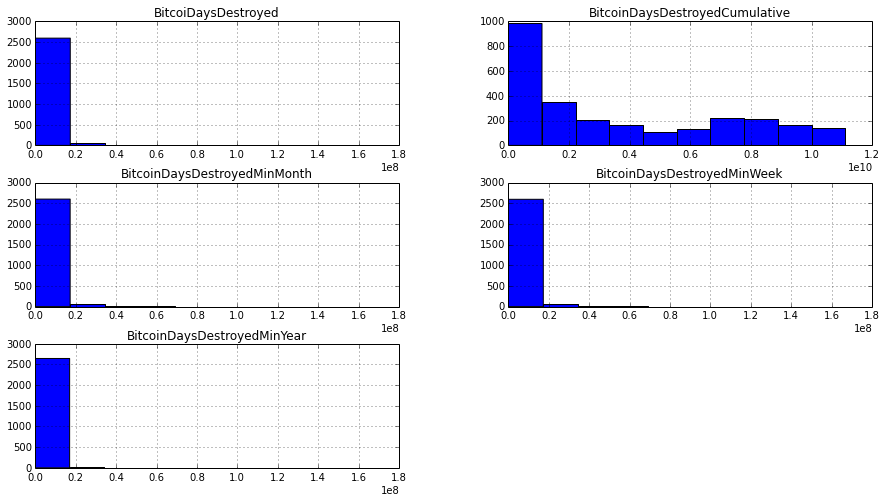
\includegraphics[width=1\linewidth]
    {gfx/bitcoin-days-destroyed-histogram}}
  \caption{Bitcoin Days Destroyed Histogram}
  \label{fig:bitcoin-days-destroyed-histogram}
\end{figure}

\begin{figure}[bth]
  \myfloatalign
  {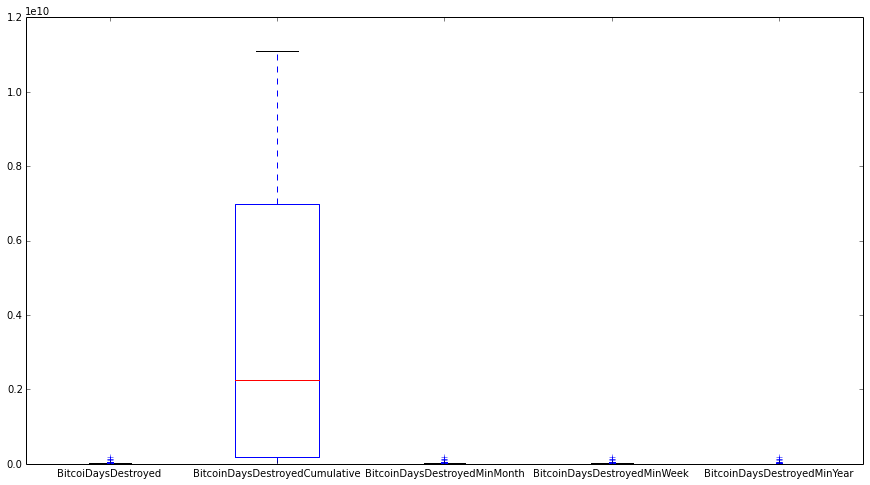
\includegraphics[width=1\linewidth]
    {gfx/bitcoin-days-destroyed-boxplot}}
  \caption{Bitcoin Days Destroyed Boxplot}
  \label{fig:bitcoin-days-destroyed-boxplot}
\end{figure}

\clearpage

%----------------------------------------------------------------------

\subsection{Bitcoin Days Destroyed Min Month}
\label{sec:bitcoin-days-destroyed-min-month}

\begin{figure}[bth]
  \myfloatalign
  {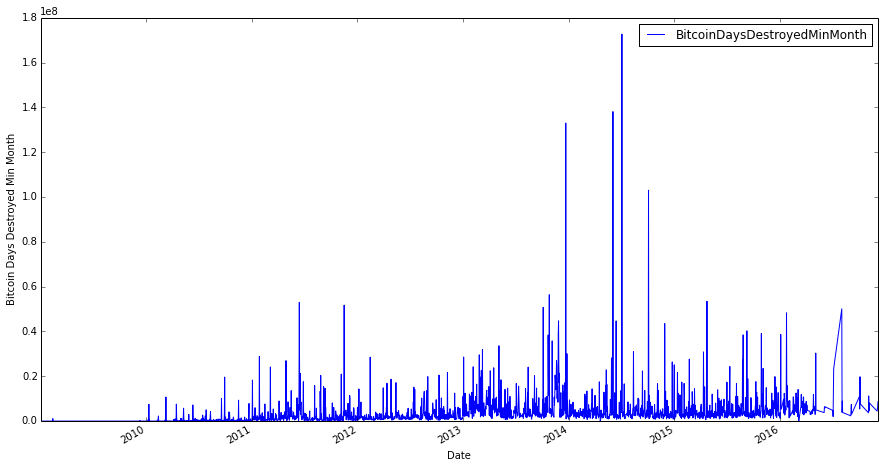
\includegraphics[width=1\linewidth]
    {gfx/bitcoin-days-destroyed-min-month-over-time}}
  \caption{Bitcoin Days Destroyed Min Month Over Time}
  \label{fig:bitcoin-days-destroyed-min-month-over-time}
\end{figure}

Bitcoin Days Destroyed filtered by minimum input age of 1 month. One
integer data point each day at 18:15:05, spanning from 03/01/2009 to
03/05/2016.  

\begin{table}
  \myfloatalign
  %\small
  \begin{tabularx}{\textwidth}{XX} 
    \toprule
    \tableheadline{Measure} & \tableheadline{Value} \\
    \midrule 
    count  & $2.679000e+03$ \\
    mean   & $3.649039e+06$ \\
    median & $1868139$      \\
    std    & $7.629002e+06$ \\
    min    & $0.000000e+00$ \\
    25\%   & $3.028175e+05$ \\
    50\%   & $1.868139e+06$ \\
    75\%   & $4.001042e+06$ \\
    max    & $1.727464e+08$ \\
    \bottomrule
  \end{tabularx}
  \caption{Statistical values for \textit{Bitcoin Days Destroyed Min Month}}
  \label{tab:bitcoin-days-destroyed-min-month}
\end{table}

\begin{figure}[bth]
  \myfloatalign
  {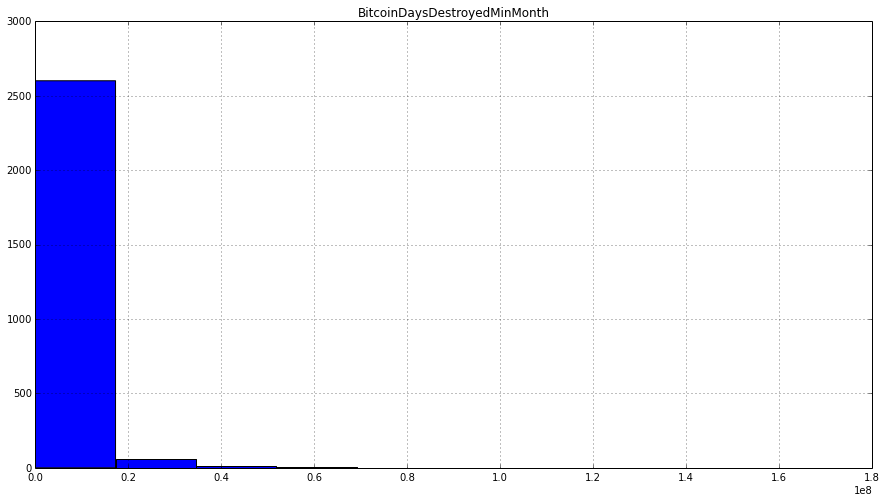
\includegraphics[width=1\linewidth]
    {gfx/bitcoin-days-destroyed-min-month-histogram}}
  \caption{Bitcoin Days Destroyed Min Month Histogram}
  \label{fig:bitcoin-days-destroyed-min-month-histogram}
\end{figure}

\begin{figure}[bth]
  \myfloatalign
  {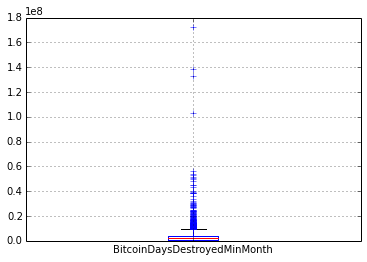
\includegraphics[width=1\linewidth]
    {gfx/bitcoin-days-destroyed-min-month-boxplot}}
  \caption{Bitcoin Days Destroyed Min Month Boxplot}
  \label{fig:bitcoin-days-destroyed-min-month-boxplot}
\end{figure}

\clearpage
%----------------------------------------------------------------------

\subsection{Bitcoin Days Destroyed Min Week}
\label{sec:bitcoin-days-destroyed-min-week}

\begin{figure}[bth]
  \myfloatalign
  {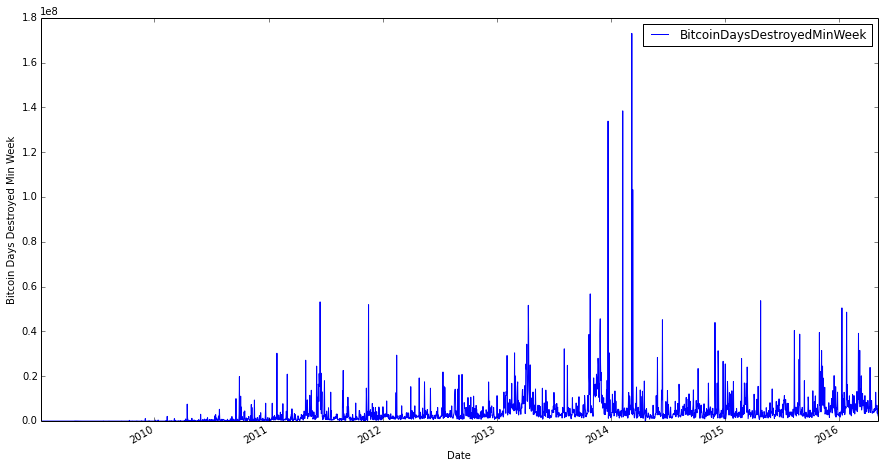
\includegraphics[width=1\linewidth]
    {gfx/bitcoin-days-destroyed-min-week-over-time}}
  \caption{Bitcoin Days Destroyed Min Week Over Time}
  \label{fig:bitcoin-days-destroyed-min-week-over-time}
\end{figure}

Bitcoin Days Destroyed filtered by minimum input age of 1 week. One
integer data point each day at 18:15:05, spanning from 03/01/2009 to
03/05/2016.

\begin{table}
  \myfloatalign
  %\small
  \begin{tabularx}{\textwidth}{XX} 
    \toprule
    \tableheadline{Measure} & \tableheadline{Value} \\
    \midrule 
    count  & $2.679000e+03$ \\
    mean   & $3.947443e+06$ \\
    median & $2210053$      \\
    std    & $7.721971e+06$ \\
    min    & $0.000000e+00$ \\
    25\%   & $4.384805e+05$ \\
    50\%   & $2.210053e+06$ \\
    75\%   & $4.454368e+06$ \\
    max    & $1.730718e+08$ \\
    \bottomrule
  \end{tabularx}
  \caption{Statistical values for \textit{Bitcoin Days Destroyed Min
      Week}} 
  \label{tab:bitcoin-days-destroyed-min-week}
\end{table}

\begin{figure}[bth]
  \myfloatalign
  {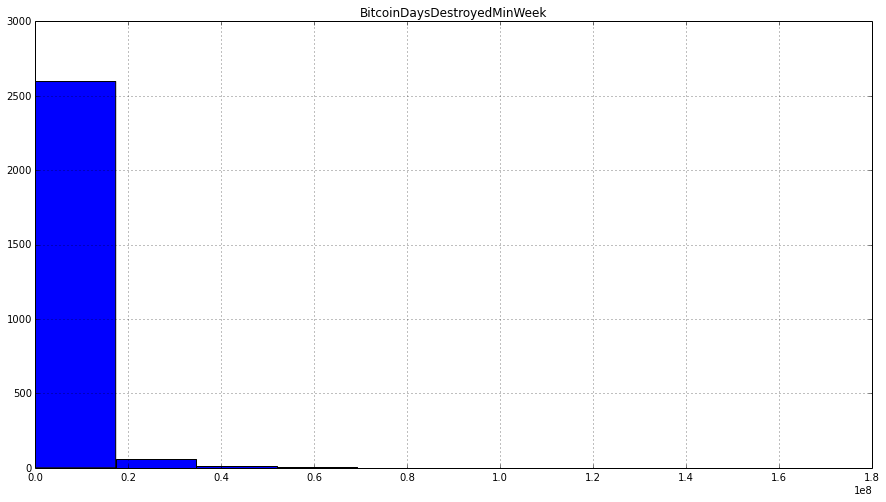
\includegraphics[width=1\linewidth]
    {gfx/bitcoin-days-destroyed-min-week-histogram}}
  \caption{Bitcoin Days Destroyed Min Week Histogram}
  \label{fig:bitcoin-days-destroyed-min-week-histogram}
\end{figure}

\begin{figure}[bth]
  \myfloatalign
  {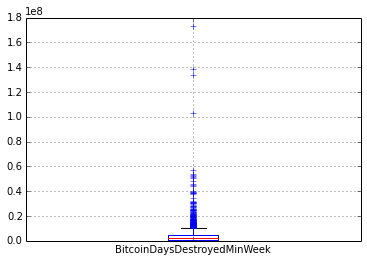
\includegraphics[width=1\linewidth]
    {gfx/bitcoin-days-destroyed-min-week-boxplot}}
  \caption{Bitcoin Days Destroyed Min Week Boxplot}
  \label{fig:bitcoin-days-destroyed-min-week-boxplot}
\end{figure}

\clearpage
%----------------------------------------------------------------------

\subsection{Bitcoin Days Destroyed Min Year}
\label{sec:bitcoin-days-destroyed-min-year}

\begin{figure}[bth]
  \myfloatalign
  {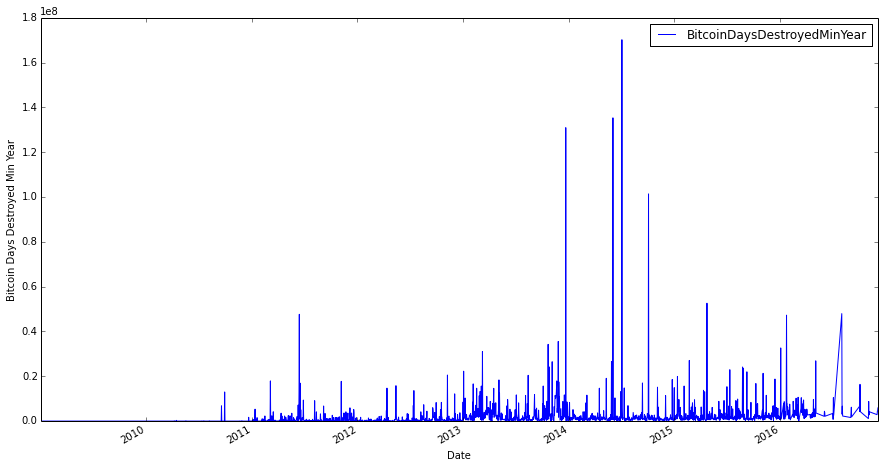
\includegraphics[width=1\linewidth]
    {gfx/bitcoin-days-destroyed-min-year-over-time}}
  \caption{Bitcoin Days Destroyed Min Year Over Time}
  \label{fig:bitcoin-days-destroyed-min-year-over-time}
\end{figure}

Bitcoin Days Destroyed filtered by minimum input age of 1 year. One
integer data point each day at 18:15:05, spanning from 03/01/2009 to
03/05/2016.

\begin{table}
  \myfloatalign
  %\small
  \begin{tabularx}{\textwidth}{XX} 
    \toprule
    \tableheadline{Measure} & \tableheadline{Value} \\
    \midrule 
    count  & $2.679000e+03$ \\
    mean   & $1.774081e+06$ \\
    median & $416483.0$     \\
    std    & $6.404385e+06$ \\
    min    & $0.000000e+00$ \\
    25\%   & $0.000000e+00$ \\
    50\%   & $4.164830e+05$ \\
    75\%   & $1.568172e+06$ \\
    max    & $1.702367e+08$ \\
    \bottomrule
  \end{tabularx}
  \caption{Statistical values for \textit{Bitcoin Days Destroyed Min
      Year}} 
  \label{tab:bitcoin-days-destroyed-min-year}
\end{table}

\begin{figure}[bth]
  \myfloatalign
  {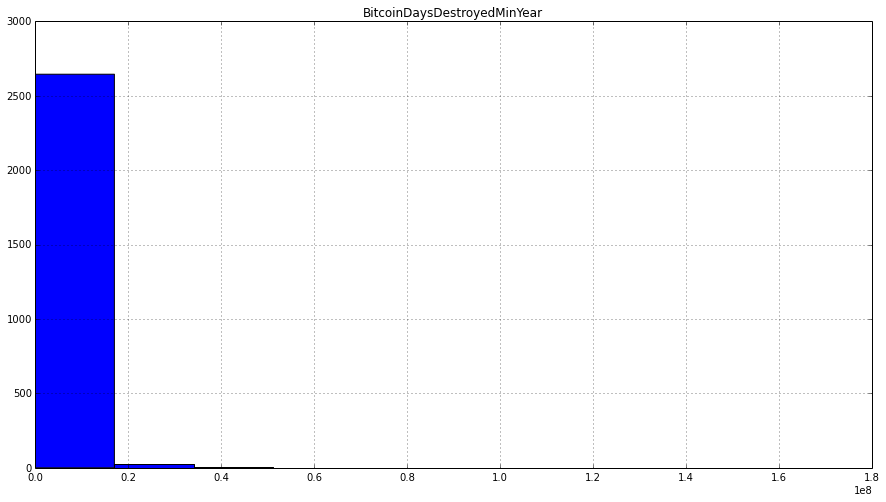
\includegraphics[width=1\linewidth]
    {gfx/bitcoin-days-destroyed-min-year-histogram}}
  \caption{Bitcoin Days Destroyed Min Year Histogram}
  \label{fig:bitcoin-days-destroyed-min-year-histogram}
\end{figure}

\begin{figure}[bth]
  \myfloatalign
  {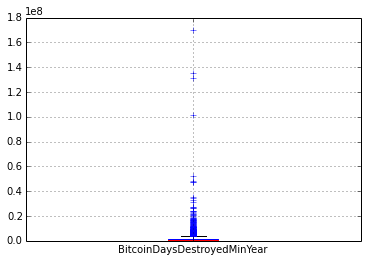
\includegraphics[width=1\linewidth]
    {gfx/bitcoin-days-destroyed-min-year-boxplot}}
  \caption{Bitcoin Days Destroyed Min Year Boxplot}
  \label{fig:bitcoin-days-destroyed-min-year-boxplot}
\end{figure}

\clearpage
%----------------------------------------------------------------------

\subsection{Bitcoin Days Destroyed Cumulative}
\label{sec:bitcoin-days-destroyed-cumulative}

\begin{figure}[bth]
  \myfloatalign
  {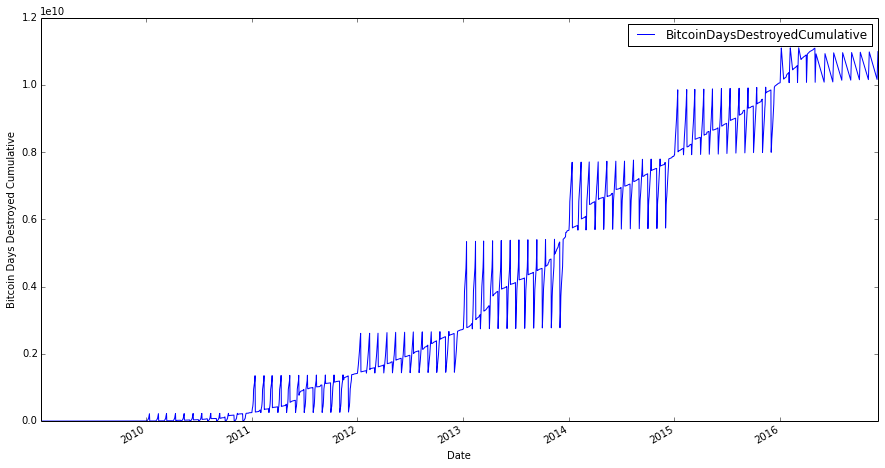
\includegraphics[width=1\linewidth]
    {gfx/bitcoin-days-destroyed-cumulative-over-time}}
  \caption{Bitcoin Days Destroyed Cumulative Over Time}
  \label{fig:bitcoin-days-destroyed-cumulative-over-time}
\end{figure}

Bitcoin Days Destroyed Cumulative acumulates all the bitcoins days
destroyed. That means that the increase of these variable shows the
increase in ``real'' transactions. In
\autoref{fig:bitcoin-days-destroyed-cumulative-over-time} we can see
that the value of this variable keeps growing, which leads us to think
that the ``real'' use of Bitcoin is also growin.

All the ``Bitcoin Days Destroyed'' variables are useful to disciminate
the ``real'' transaction between people and the rapid transaction
that can be done by traders for example.

The dataset comprises one integer data point each day, at
18:15:05, spanning from 03/01/2009 to 03/05/2016.

\begin{table}
  \myfloatalign
  %\small
  \begin{tabularx}{\textwidth}{XX} 
    \toprule
    \tableheadline{Measure} & \tableheadline{Value} \\
    \midrule 
    count  & $2.679000e+03$ \\
    mean   & $3.609471e+09$ \\
    median & $2265772771.0$ \\
    std    & $3.572547e+09$ \\
    min    & $0.000000e+00$ \\
    25\%   & $1.817693e+08$ \\
    50\%   & $2.265773e+09$ \\
    75\%   & $6.971917e+09$ \\
    max    & $1.110959e+10$ \\ 
    \bottomrule
  \end{tabularx}
  \caption{Statistical values for \textit{Bitcoin Days Destroyed Cumulative}}
  \label{tab:bitcoin-days-destroyed-cumulative}
\end{table}

\begin{figure}[bth]
  \myfloatalign
  {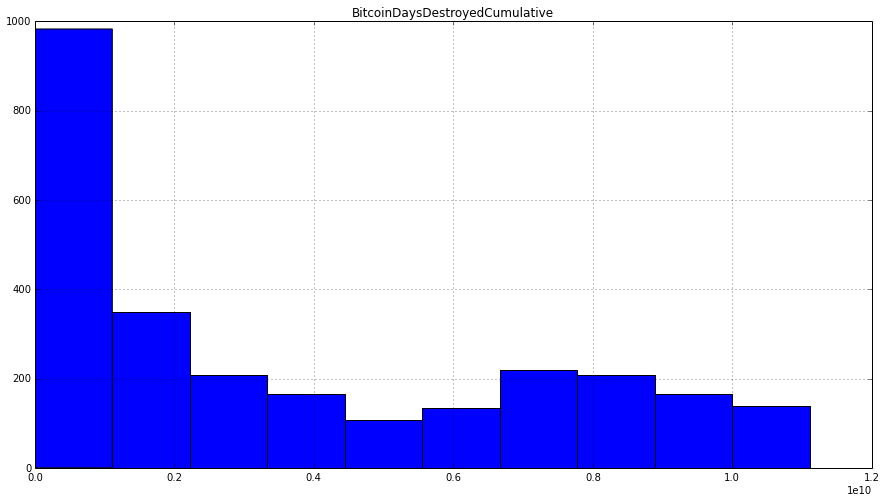
\includegraphics[width=1\linewidth]
    {gfx/bitcoin-days-destroyed-cumulative-histogram}}
  \caption{Bitcoin Days Destroyed Cumulative Histogram}
  \label{fig:bitcoin-days-destroyed-cumulative-histogram}
\end{figure}

\begin{figure}[bth]
  \myfloatalign
  {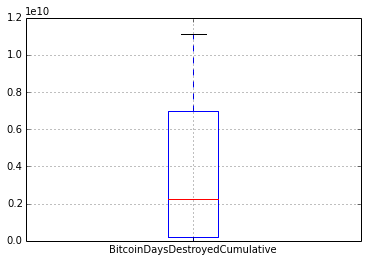
\includegraphics[width=1\linewidth]
    {gfx/bitcoin-days-destroyed-cumulative-boxplot}}
  \caption{Bitcoin Days Destroyed Cumulative Boxplot}
  \label{fig:bitcoin-days-destroyed-cumulative-boxplot}
\end{figure}

\clearpage
%----------------------------------------------------------------------

\subsection{Block Size}
\label{sec:block-size}

\begin{figure}[bth]
  \myfloatalign
  {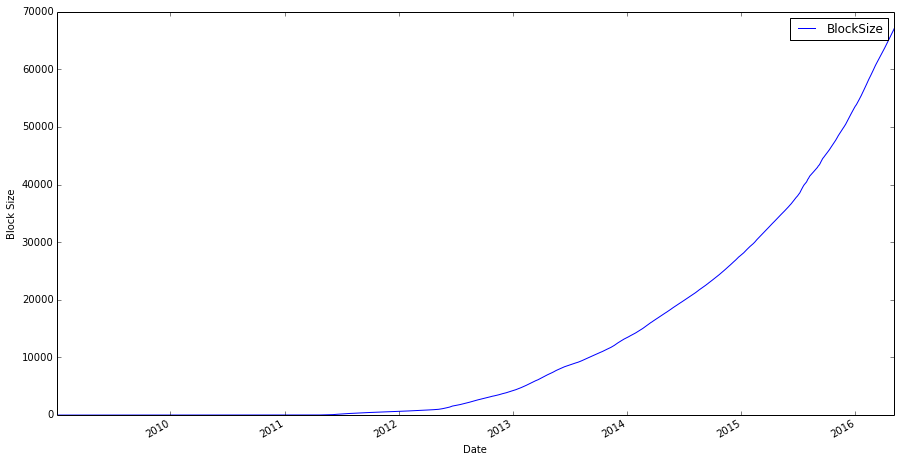
\includegraphics[width=1\linewidth]
    {gfx/block-size-over-time}}
  \caption{Block Size Over Time}
  \label{fig:block-size-over-time}
\end{figure}

The total size (in MB) of all block headers and transactions. Not
including database indexes. One real number data point each day, at
18:15:05, spanning from 03/01/2009 to 03/05/2016.

The total block size is increasing exponentialy as seen in
\autoref{fig:block-size-over-time}. This basically represents that the
total ammount of transactions are increasing at that rate.

\begin{table}
  \myfloatalign
  %\small
  \begin{tabularx}{\textwidth}{XX} 
    \toprule
    \tableheadline{Measure} & \tableheadline{Value} \\
    \midrule 
    count  & $2678.000000$       \\
    mean   & $9.727391$          \\
    median & $6.219650292785771$ \\
    std    & $13.268846$         \\
    min    & $0.000000$          \\
    25\%   & $1.301186$          \\
    50\%   & $6.219650$          \\
    75\%   & $10.401306$         \\
    max    & $90.202095$         \\
    \bottomrule
  \end{tabularx}
  \caption{Statistical values for \textit{Block Size}}
  \label{tab:block-size}
\end{table}

\begin{figure}[bth]
  \myfloatalign
  {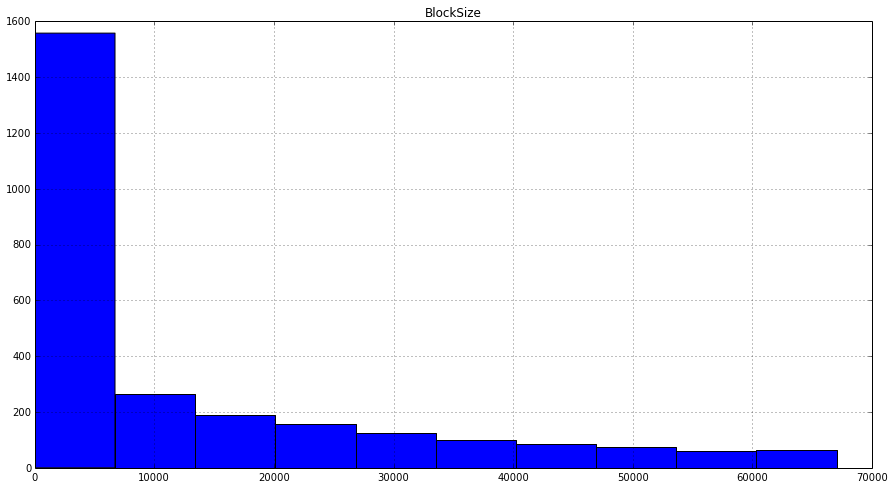
\includegraphics[width=1\linewidth]
    {gfx/block-size-histogram}}
  \caption{Block Size Histogram}
  \label{fig:block-size-histogram}
\end{figure}

\begin{figure}[bth]
  \myfloatalign
  {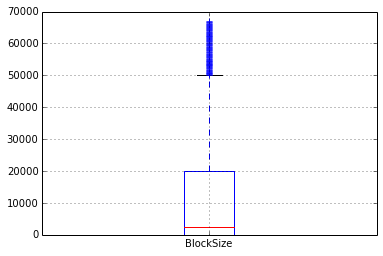
\includegraphics[width=1\linewidth]
    {gfx/block-size-boxplot}}
  \caption{Block Size Boxplot}
  \label{fig:block-size-boxplot}
\end{figure}

\clearpage
%----------------------------------------------------------------------

\subsection{Cost Per Transaction}
\label{sec:cost-per-transaction}

This variable shows miners revenue (in USD) divided by the number of
transactions. To better understand the fluctuations of \textit{Cost
  Per Transaction} show in
\autoref{fig:cost-per-transaction-over-time} we include the next
definition, found
\href{https://en.bitcoin.it/wiki/Transaction_fees}{here}:

\textit{``The transaction fee is processed by and received by the
  bitcoin miner. When a new bitcoin block is generated with a
  successful hash, the information for all of the transactions is
  included with the block and all transaction fees are collected by
  that user creating the block, who is free to assign those fees to
  himself.}

\textit{Transaction fees are voluntary on the part of the person
  making the bitcoin transaction, as the person attempting to make a
  transaction can include any fee or none at all in the transaction.
  On the other hand, nobody mining new bitcoins necessarily needs to
  accept the transactions and include them in the new block being
  created. The transaction fee is therefore an incentive on the part
  of the bitcoin user to make sure that a particular transaction will
  get included into the next block which is generated.''}

Knowing how the fees work in Bitcoin, we can see that the cost depends
on the will of the miner to accept or not the transaction. If we look
at \autoref{fig:n-transactions-multiple-over-time} we can see that
there is some correlation between the number of transactions been
processed and the cost of each transaction. The first peek in both
figures coincide around January/2011, after that, in mid 2011 there is
a sustained increase in the number of transactions, which in
\autoref{fig:cost-per-transaction-over-time} has a counterpart peek in
the cost of transactions, probably, because a lot of people wanted to
make transactions and the amount of miners were small. After that the
cost per transaction lowers and doesn't have a significant increase
till mid 2013. This increase is due to an increase in trade volume,
that can be seen clearly in \autoref{fig:trade-volume-over-time}. Next
to that, we see the biggest cost of cost per transaction so far, which
took place in the end of 2013 and start of 2014. This peek also occurs
simultaneously to a trade volume peek.

\begin{figure}[bth]
  \myfloatalign
  {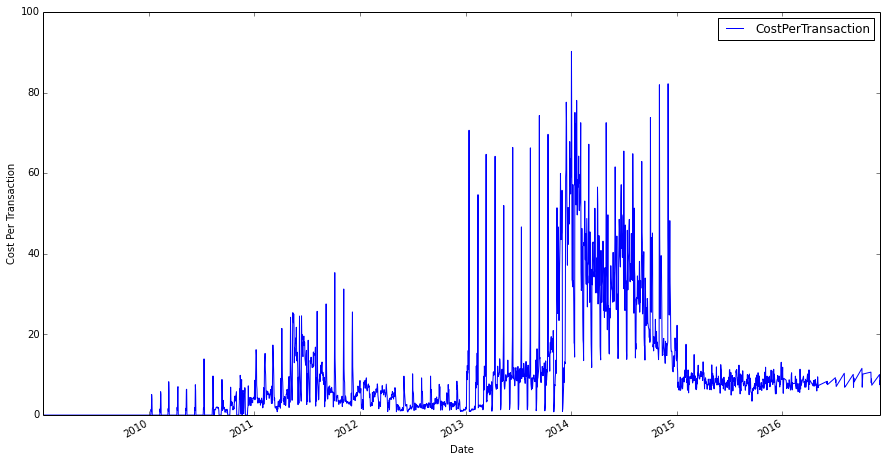
\includegraphics[width=1\linewidth]
    {gfx/cost-per-transaction-over-time}}
  \caption{Cost Per Transaction Over Time}
  \label{fig:cost-per-transaction-over-time}
\end{figure}

The dataset comprises one real number data point each day, at
18:15:05, spanning from 03/01/2009 to 03/05/2016.

\begin{table}
  \myfloatalign
  %\small
  \begin{tabularx}{\textwidth}{XX} 
    \toprule
    \tableheadline{Measure} & \tableheadline{Value} \\
    \midrule 
    count  & $2678$ \\
    mean   & $9.727391$    \\
    median & $6.21965$     \\
    std    & $13.268846$   \\
    min    & $0$    \\
    $25$\  & $1.301186$    \\
    $50$\  & $6.219650$    \\
    $75$\  & $10.401306$   \\
    max    & $90.202095$   \\
    \bottomrule
  \end{tabularx}
  \caption{Statistical values for \textit{Cost Per Transaction}}
  \label{tab:cost-per-transaction}
\end{table}

\begin{figure}[bth]
  \myfloatalign
  {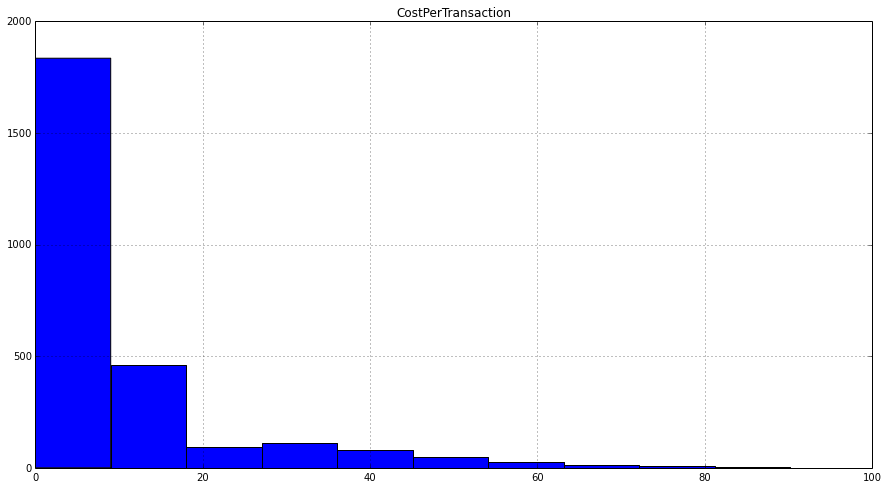
\includegraphics[width=1\linewidth]
    {gfx/cost-per-transaction-histogram}}
  \caption{Cost Per Transaction Histogram}
  \label{fig:cost-per-transaction-histogram}
\end{figure}

\begin{figure}[bth]
  \myfloatalign
  {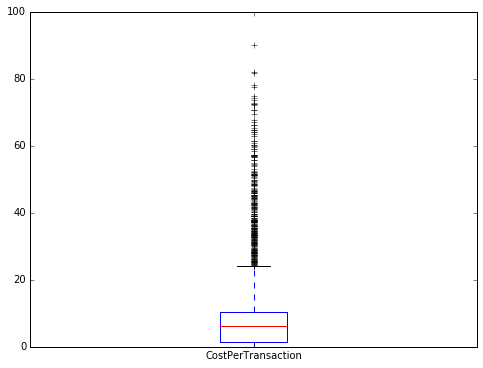
\includegraphics[width=1\linewidth]
    {gfx/cost-per-transaction-boxplot}}
  \caption{Cost Per Transaction Boxplot}
  \label{fig:cost-per-transaction-boxplot}
\end{figure}

\clearpage
%----------------------------------------------------------------------

\subsection{Cost Per Transaction Percent}
\label{sec:cost-per-transaction-percent}

\begin{figure}[bth]
  \myfloatalign
  {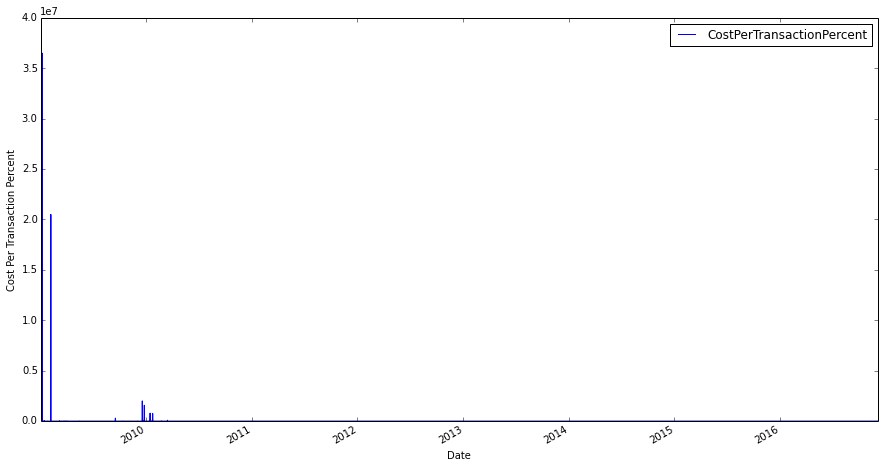
\includegraphics[width=1\linewidth]
    {gfx/cost-per-transaction-percent-over-time}}
  \caption{Cost Per Transaction Percent Over Time}
  \label{fig:cost-per-transaction-percent-over-time}
\end{figure}

This variable shows miners revenue as percentage of the transaction
volume. Basically what
\autoref{fig:cost-per-transaction-percent-over-time} shows is that
over time, the transactions fees are decreasing with respect to the
transaction amount itself. The median, shown in
\autoref{tab:cost-per-transaction-percent}, is $3.283375136886966\%$,
which reflects the percent of transaction that is used mostly in all
Bitcoin transactions.

The dataset comprises one real number data point each day, at
18:15:05, spanning from 03/01/2009 to 03/05/2016.

\begin{table}
  \myfloatalign
  %\small
  \begin{tabularx}{\textwidth}{XX} 
    \toprule
    \tableheadline{Measure} & \tableheadline{Value} \\
    \midrule 
    count  & $2678.000000$       \\
    mean   & $23603.541449$      \\
    median & $3.283375136886966$ \\
    std    & $810554.930805$     \\
    min    & $0.000000$          \\
    25\%   & $1.580112$          \\
    50\%   & $3.283375$          \\
    75\%   & $9.606991$          \\
    max    & $36500000.000000$   \\
    \bottomrule
  \end{tabularx}
  \caption{Statistical values for \textit{Cost Per Transaction Percent}}
  \label{tab:cost-per-transaction-percent}
\end{table}

\begin{figure}[bth]
  \myfloatalign
  {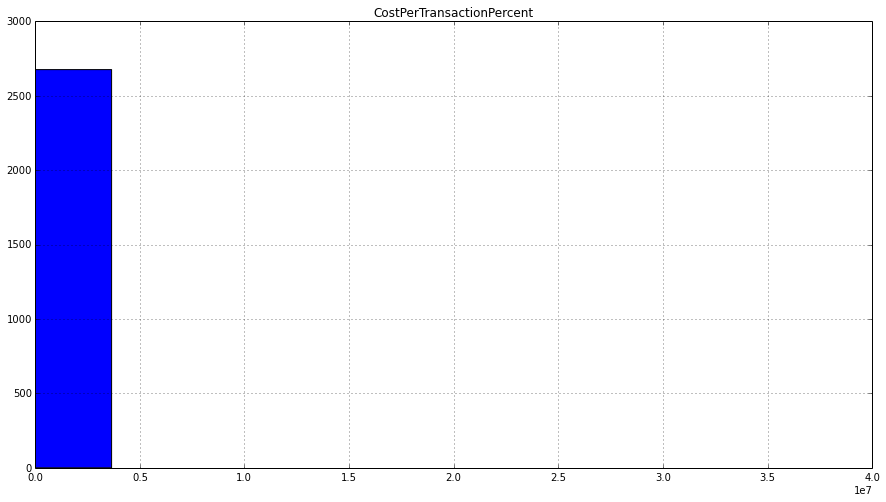
\includegraphics[width=1\linewidth]
    {gfx/cost-per-transaction-percent-histogram}}
  \caption{Cost Per Transaction Percent Histogram}
  \label{fig:cost-per-transaction-percent-histogram}
\end{figure}

\begin{figure}[bth]
  \myfloatalign
  {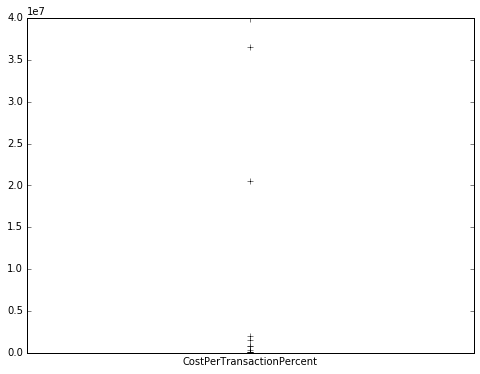
\includegraphics[width=1\linewidth]
    {gfx/cost-per-transaction-percent-boxplot}}
  \caption{Cost Per Transaction Percent Boxplot}
  \label{fig:cost-per-transaction-percent-boxplot}
\end{figure}

\clearpage
%----------------------------------------------------------------------

\subsection{Difficulty}
\label{sec:difficulty}

\begin{figure}[bth]
  \myfloatalign
  {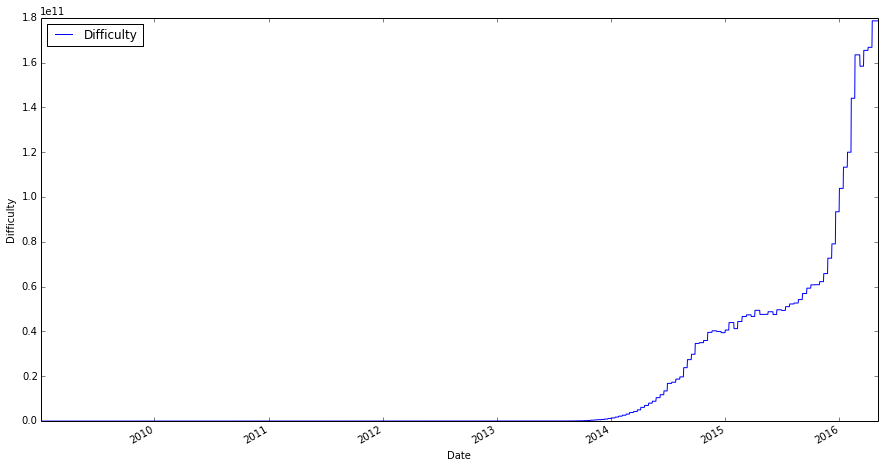
\includegraphics[width=1\linewidth]
    {gfx/difficulty-over-time}}
  \caption{Difficulty Over Time}
  \label{fig:difficulty-over-time}
\end{figure}

A relative measure of how difficult it is to find a new block. The
difficulty is adjusted periodically as a function of how much hashing
power has been deployed by the network of miners. That can be seen
looking at how similar are \autoref{fig:difficulty-over-time} and
\autoref{fig:hash-rate-over-time}. The graphic representing the
difficulty has a discrete shape, that is because the difficulty is
adjusted automatically every 2016 blocks, and changes equally for the
entire Bitcoin network. Until 2014, the difficulty of mining was
very low, it started to raise probably because the trade volume in the
end of 2013 and start of 2014 was approximately 70.000.000\$, which
attracted professional miners with a greater processing power, those
creating more and more blocks and augmenting the difficulty of mining.

The dataset comprises one real number data point each day, at
18:15:05, spanning from 03/01/2009 to 03/05/2016.

\begin{table}
  \myfloatalign
  %\small
  \begin{tabularx}{\textwidth}{XX} 
    \toprule
    \tableheadline{Measure} & \tableheadline{Value} \\
    \midrule 
    count  & $2.678000e+03$      \\
    mean   & $1.683580e+10$      \\
    median & $2440642.606915964$ \\
    std    & $3.561708e+10$      \\
    min    & $0.000000e+00$      \\
    25\%   & $3.091737e+03$      \\
    50\%   & $2.440643e+06$      \\
    75\%   & $1.681846e+10$      \\
    max    & $1.786783e+11$      \\
    \bottomrule
  \end{tabularx}
  \caption{Statistical values for \textit{Difficulty}}
  \label{tab:difficulty}
\end{table}

\begin{figure}[bth]
  \myfloatalign
  {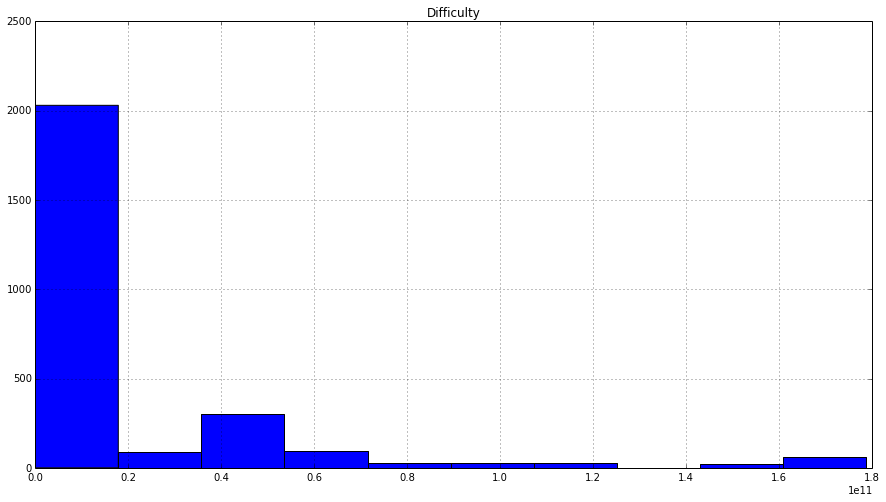
\includegraphics[width=1\linewidth]
    {gfx/difficulty-histogram}}
  \caption{Difficulty Histogram}
  \label{fig:difficulty-histogram}
\end{figure}

\begin{figure}[bth]
  \myfloatalign
  {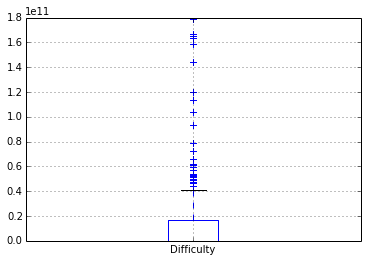
\includegraphics[width=1\linewidth]
    {gfx/difficulty-boxplot}}
  \caption{Difficulty Boxplot}
  \label{fig:difficulty-boxplot}
\end{figure}

\clearpage
%----------------------------------------------------------------------

\subsection{Estimated Transaction Volume}
\label{sec:estimated-transaction-volume}

\begin{figure}[bth]
  \myfloatalign
  {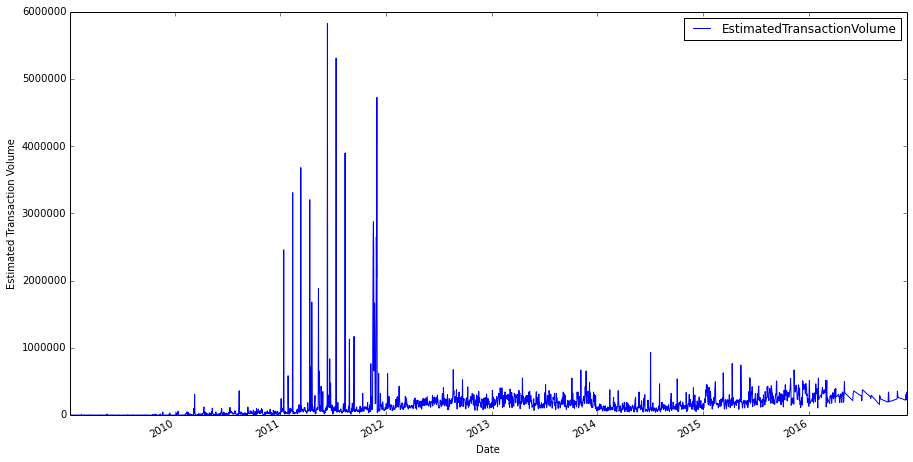
\includegraphics[width=1\linewidth]
    {gfx/estimated-transaction-volume-over-time}}
  \caption{Estimated Transaction Volume Over Time}
  \label{fig:estimated-transaction-volume-over-time}
\end{figure}

The total estimated value of transactions on the Bitcoin blockchain
(does not include coins returned to sender as change). The transaction
volume represented in
\autoref{fig:estimated-transaction-volume-over-time} is very slowly
increasing, meaning that more transactions in Bitcoin are processed.
However, it doesn't represent the actual value of transactions,
because people think in their local currency when trading or shopping,
and Bitcoin's value is volatile. Is more useful the next variable,
\textit{Estimated Transaction Volume USD} that gives as tells the
actual value of transactions. The peak that happened in 2012 wouldn't
occur easily today due to the current value of Bitcoin.

The data-set comprises one integer data point each day, at
18:15:05, spanning from 03/01/2009 to 03/05/2016.

\begin{table}
  \myfloatalign
  %\small
  \begin{tabularx}{\textwidth}{XX} 
    \toprule
    \tableheadline{Measure} & \tableheadline{Value} \\
    \midrule 
    count  & $2679.000000$    \\
    mean   & $157340.920119$  \\
    median & $118843.0$       \\
    std    & $282285.024788$  \\
    min    & $0.000000$       \\
    $25$\% & $30553.000000$   \\
    $50$\% & $118843.000000$  \\
    $75$\% & $210442.000000$  \\
    max    & $5825066.000000$ \\
    \bottomrule
  \end{tabularx}
  \caption{Statistical values for \textit{Estimated Transaction Volume}}
  \label{tab:estimated-transaction-volume}
\end{table}

\begin{figure}[bth]
  \myfloatalign
  {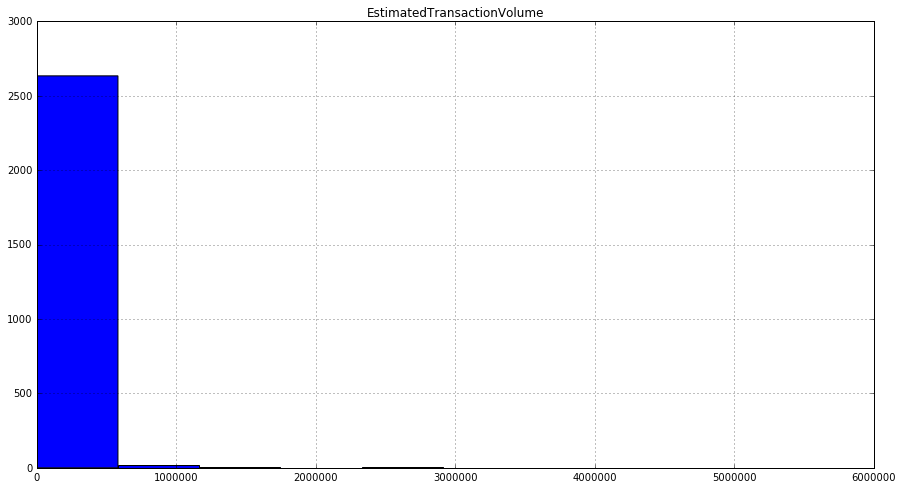
\includegraphics[width=1\linewidth]
    {gfx/estimated-transaction-volume-histogram}}
  \caption{Estimated Transaction Volume Histogram}
  \label{fig:estimated-transaction-volume-histogram}
\end{figure}

\begin{figure}[bth]
  \myfloatalign
  {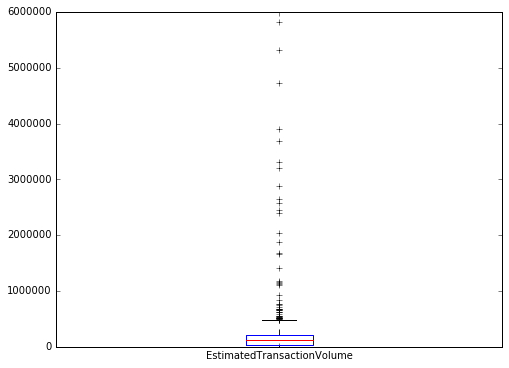
\includegraphics[width=1\linewidth]
    {gfx/estimated-transaction-volume-boxplot}}
  \caption{Estimated Transaction Volume Boxplot}
  \label{fig:estimated-transaction-volume-boxplot}
\end{figure}

\clearpage
%----------------------------------------------------------------------

\subsection{Estimated Transaction Volume USD}
\label{sec:estimated-transaction-volume-usd}

\begin{figure}[bth]
  \myfloatalign
  {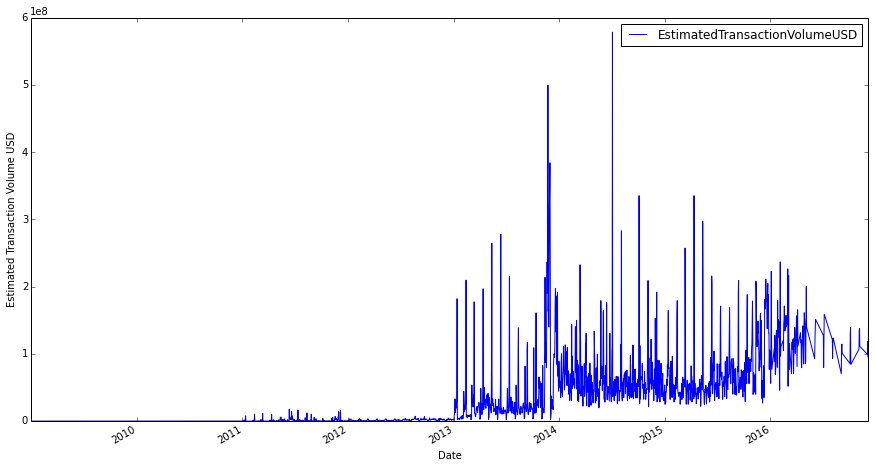
\includegraphics[width=1\linewidth]
    {gfx/estimated-transaction-volume-usd-over-time}}
  \caption{Estimated Transaction Volume USD Over Time}
  \label{fig:estimated-transaction-volume-usd-over-time}
\end{figure}

The Estimated Transaction Volume in USD value, shown in
\autoref{fig:estimated-transaction-volume-usd-over-time}, can be
explained by the average value of Bitcoin, shown in
\autoref{fig:market-price-over-time}, because nearly all the events
are paired in the two figures. There is a small increase in estimated
transaction volume in USD in mid 2011 at the same time than the
average price of Bitcoin increases. Later on, in 2013 there is a
bigger increase in estimated volume that is also reflected in the
average price. Then we have the two biggest peaks around January of
2014 coinciding with the higher average value of Bitcoin (also
represented in two peaks). After that there is decrease in average
price and estimated volume till 2016 where Bitcoin average price
starts to increase at the same time that the estimate transaction
volume increases.

This data-set comprises one integer data point each day, at 18:15:05,
spanning from 03/01/2009 to 03/05/2016.

\begin{table}
  \myfloatalign
  %\small
  \begin{tabularx}{\textwidth}{XX} 
    \toprule
    \tableheadline{Measure} & \tableheadline{Value} \\
    \midrule 
    count  & $2.679000e+03$ \\
    median & $2481424.0$    \\
    mean   & $3.018470e+07$ \\
    std    & $4.923048e+07$ \\
    min    & $0.000000e+00$ \\
    $25$\% & $5.086000e+03$ \\
    $50$\% & $2.481424e+06$ \\
    $75$\% & $4.761785e+07$ \\
    max    & $5.787707e+08$ \\
    \bottomrule
  \end{tabularx}
  \caption{Statistical values for \textit{Estimated Transaction Volume USD}}
  \label{tab:estimated-transaction-volume-usd}
\end{table}

\begin{figure}[bth]
  \myfloatalign
  {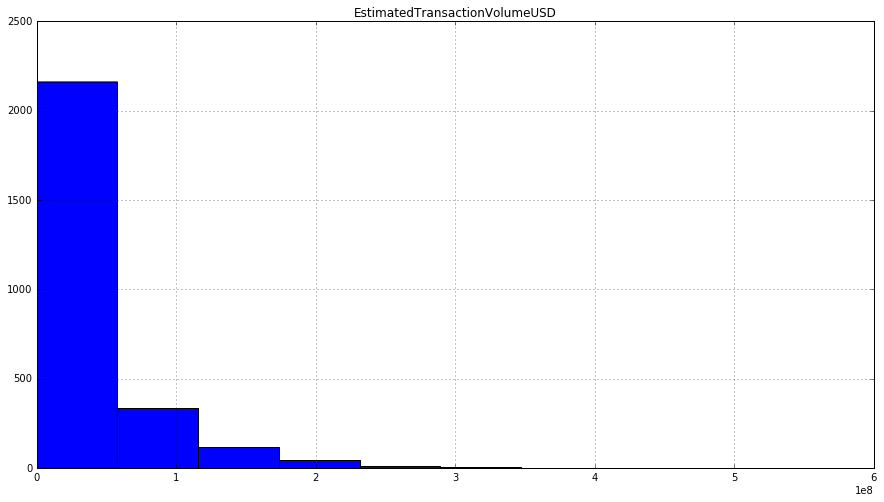
\includegraphics[width=1\linewidth]
    {gfx/estimated-transaction-volume-usd-histogram}}
  \caption{Estimated Transaction Volume USD Histogram}
  \label{fig:estimated-transaction-volume-usd-histogram}
\end{figure}

\begin{figure}[bth]
  \myfloatalign
  {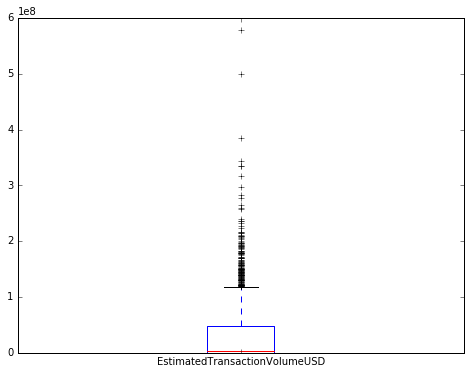
\includegraphics[width=1\linewidth]
    {gfx/estimated-transaction-volume-usd-boxplot}}
  \caption{Estimated Transaction Volume USD Boxplot}
  \label{fig:estimated-transaction-volume-usd-boxplot}
\end{figure}

\clearpage

%----------------------------------------------------------------------

\subsection{Euro price in USD}
\label{sec:euro-price-in-usd}

\begin{figure}[bth]
  \myfloatalign
  {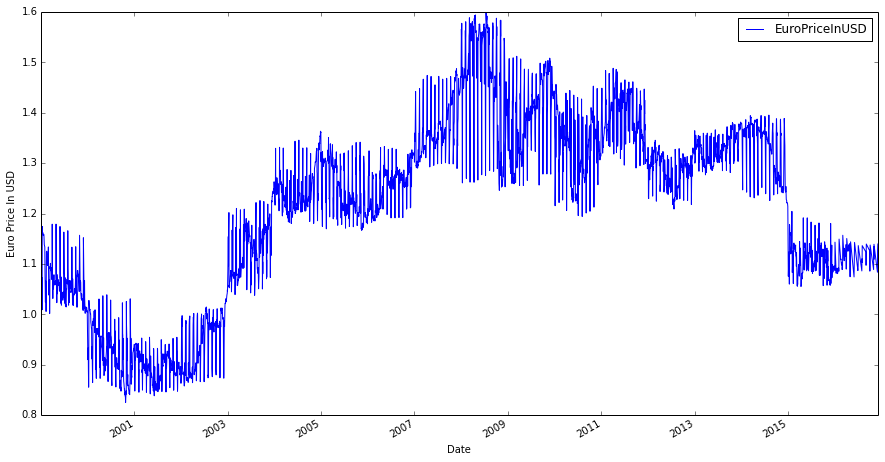
\includegraphics[width=1\linewidth]
    {gfx/euro-price-in-usd-over-time}} 
  \caption{Euro price in USD Over Time}
  \label{fig:euro-price-in-usd-over-time}
\end{figure}

Euro price in USD provided by the European Central Bank from the
creation of the Euro. One real data entry per day, spanning from
04/01/1999 to 10/05/2016.

This dataset has latent values. We have used interpolation in order to
fill the missing values.

As shown in \autoref{fig:euro-price-in-usd-over-time} the value of Euro
has been above that of the USD from its creation, been the period of
2000 through 2003 its closer price to each other. From 2003 to 2007
the price of the Euro increased, coinciding with an increase on the
interest imposed by the BCE. This increase in the interest of the
credits is followed by the collapse of the housing bubble in 2007,
where the price of the Euro kept increasing, altough the interest was
maintained by the BCE until 2009 where the BCE started to lower it.
The increase in the Euro price is probably due to strategies of the
Federal Reserve to lower the price of the USD. Finally in 2015, the
BCE lowered the interests of credits approaching the $0.0\%$, and
that's reflected with a decrease in the price of the Euro with respect
to USD.

\begin{table}
  \myfloatalign
  %\small
  \begin{tabularx}{\textwidth}{XX} 
    \toprule
    \tableheadline{Measure} & \tableheadline{Value} \\
    \midrule 
    count & 4443\\
    mean  & 1.216306\\
    median & 1.2579\\
    std   & 0.177679\\
    min   & 0.825200\\
    25\%  & 1.088300\\
    50\%  & 1.257900\\
    75\%  & 1.345050\\
    max   & 1.599000\\
    \bottomrule
  \end{tabularx}
  \caption{Statistical values for \textit{Euro price in USD}}
  \label{tab:euro-price-in-usd}
\end{table}

There are 62 missing values in the data which has been interpolated
after obtaining the descriptive variables of
\autoref{tab:euro-price-in-usd}

\begin{figure}[bth]
  \myfloatalign
  {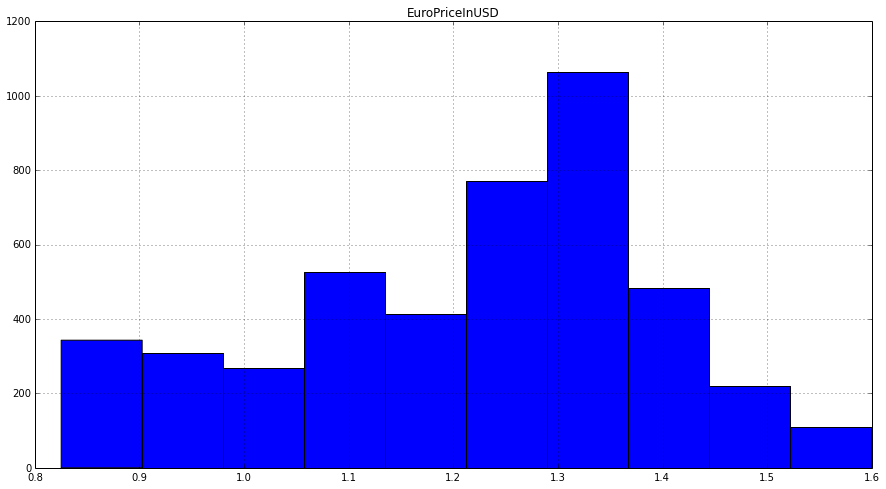
\includegraphics[width=1\linewidth]
    {gfx/euro-price-in-usd-histogram}} 
  \caption{Euro price in USD Histogram}
  \label{fig:euro-price-in-usd-histogram}
\end{figure}

\begin{figure}[bth]
  \myfloatalign
  {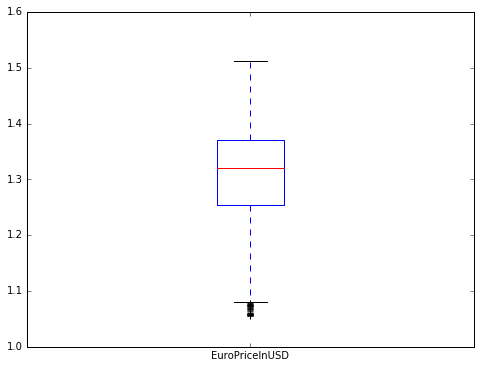
\includegraphics[width=1\linewidth]
    {gfx/euro-price-in-usd-boxplot}}
  \caption{Euro price in USD Boxplot}
  \label{fig:euro-price-in-usd-boxplot}
\end{figure}

\clearpage

%----------------------------------------------------------------------

\subsection{Hash Rate}
\label{sec:hash-rate}

\begin{figure}[bth]
  \myfloatalign
  {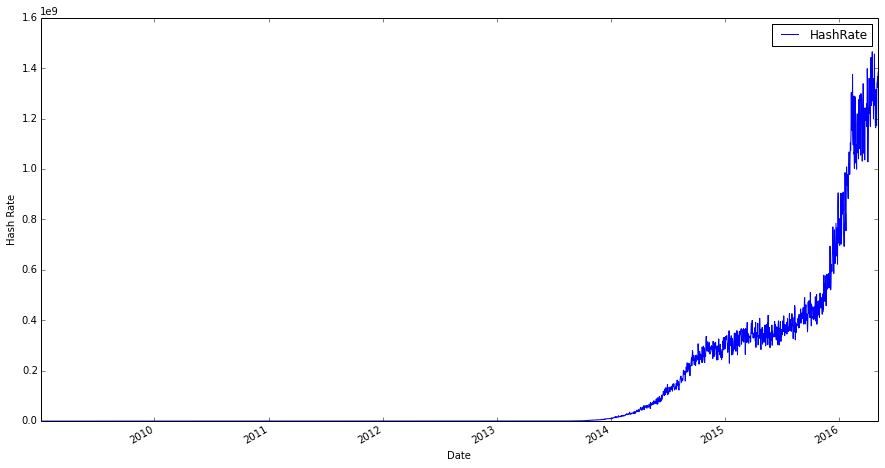
\includegraphics[width=1\linewidth]
    {gfx/hash-rate-over-time}}
  \caption{Hash Rate Over Time}
  \label{fig:hash-rate-over-time}
\end{figure}

The estimated number of giga hashes per second (billions of hashes per
second) the Bitcoin network is performing. The chart in
\autoref{fig:hash-rate-over-time} shows us how mining really started
when Bitcoin raised to its highest value around 2014, reaching more
than 1000\$ per BTC. From that point on, the processing to mining has
increased at approximately $0.2 \times 10^9$ hashes per second, and in
2016, at the same time that the Bitcoin price is starting to increase,
the hash rate started to grow at $1 \times 10^9$ hashes per second in
just a few months. 

This data-set comprises one real number data point each day, at
18:15:05, spanning from 03/01/2009 to 03/05/2016.

\begin{table}
  \myfloatalign
  %\small
  \begin{tabularx}{\textwidth}{XX}
    \toprule
    \tableheadline{Measure} & \tableheadline{Value} \\
    \midrule
    count  & $2.678000e+03$      \\
    mean   & $1.265485e+08$      \\
    median & $19063.08687085293$ \\
    std    & $2.683517e+08$      \\
    min    & $0.000000e+00$      \\
    $25$\% & $2.973922e+01$      \\
    $50$\% & $1.906309e+04$      \\
    $75$\% & $1.250993e+08$      \\
    max    & $1.465554e+09$      \\
    \bottomrule
  \end{tabularx}
  \caption{Statistical values for \textit{Hash Rate}}
  \label{tab:hash-rate}
\end{table}

\begin{figure}[bth]
  \myfloatalign
  {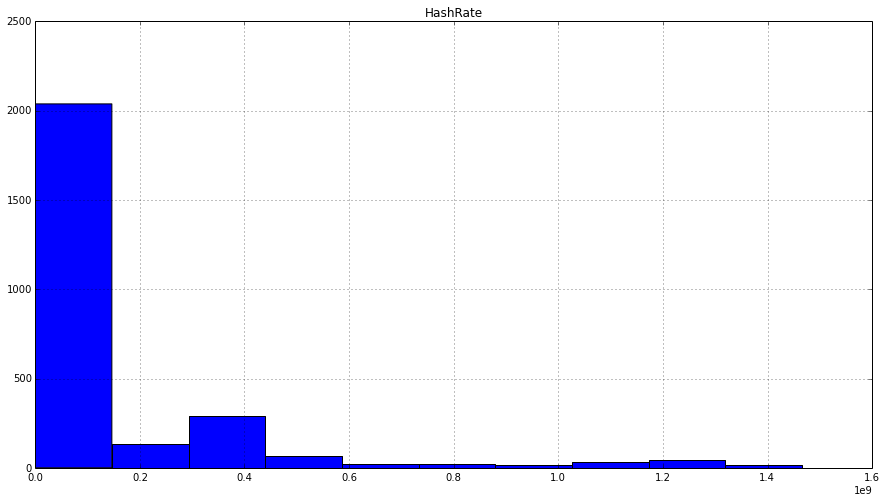
\includegraphics[width=1\linewidth]
    {gfx/hash-rate-histogram}}
  \caption{Hash Rate Histogram}
  \label{fig:hash-rate-histogram}
\end{figure}

\begin{figure}[bth]
  \myfloatalign
  {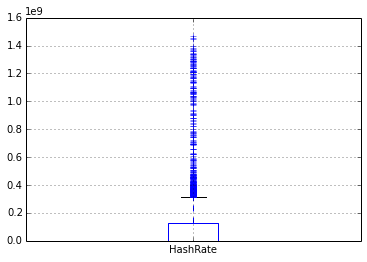
\includegraphics[width=1\linewidth]
    {gfx/hash-rate-boxplot}}
  \caption{Hash Rate Boxplot}
  \label{fig:hash-rate-boxplot}
\end{figure}

\clearpage
%----------------------------------------------------------------------

\subsection{Market Capitalization}
\label{sec:market-cap}

\begin{figure}[bth]
  \myfloatalign
  {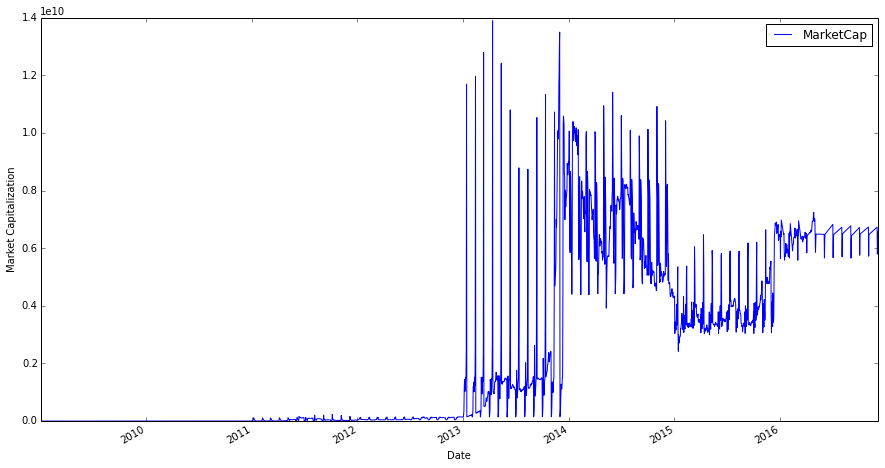
\includegraphics[width=1\linewidth]
    {gfx/market-cap-over-time}}
  \caption{Market Capitalization Over Time}
  \label{fig:market-cap-over-time}
\end{figure}

The total USD value of bitcoin supply in circulation, as calculated by
the daily average market price across major exchanges. This variable
is related to many others, starting with the Bitcoin market price,
with is virtually the same as this one, the number of transactions,
that can explain the fluctuations in the Bitcoin price and different
events. In March 9, 2011, the Bitcoin reaches parity with USD which is
shown in a timid growth in market capitalization followed by a
decrease. After that there isn't a big growth until 2013, where
several things happen, Mega, the cloud storage service, starts
accepting Bitcoins, Internet Archive starts accepting Bitcoins, a new
food service \href{PizzaForCoins.com}{PizzaForCoins.com} accepts
Bitcoins as a payment for food, CoinDesk is launched by Spotify
investor and Coinbase receives 5 million USD in funding. This, and
several other events increase the market capitalization for Bitcoin.

After that there is a decrease in market capitalization of Bitcoin,
maybe because MtGox, the largest exchange operator at the time, was
seized by The United States Department of Homeland Security.

In the second half of 2013, various events happen that can be the
cause of the raise of Bitcoin market capitalization, first, in August
6th, Bitcoin is ruled currency by a Texas judge, then in August 20th,
Bitcoin is ruled as private money in Germany, then in August 28th,
RoboCoin, a Bitcoin ATM manufacturer, starts accepting orders. This
can be the cause of the huge peek at the end of 2013 and start of
2014. There are no clear events in the Bitcoin history that explain
the period after 2014, which leads us to think that the price has been
fluctuating due to trading strategies.

This data-set comprises one real number data point each day, at
18:15:05, spanning from 03/01/2009 to 03/05/2016.

\begin{table}
  \myfloatalign
  %\small
  \begin{tabularx}{\textwidth}{XX} 
    \toprule
    \tableheadline{Measure} & \tableheadline{Value} \\
    \midrule 
    count  & $2.678e+03$     \\
    mean   & $2.072915e+09$  \\
    median & $115624066.175$ \\
    std    & $2.879009e+09$  \\
    min    & $0$             \\
    $25$\% & $1.00547e+06$   \\
    $50$\% & $1.156241e+08$  \\
    $75$\% & $3.850512e+09$  \\
    max    & $1.390005e+10$  \\
    \bottomrule
  \end{tabularx}
  \caption{Statistical values for \textit{Market Capitalization}}
  \label{tab:market-cap}
\end{table}

\begin{figure}[bth]
  \myfloatalign
  {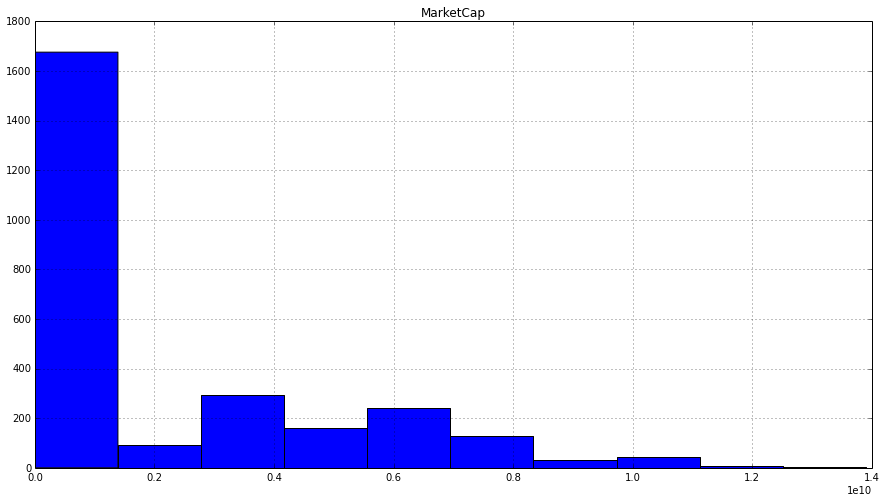
\includegraphics[width=1\linewidth]
    {gfx/market-cap-histogram}}
  \caption{Market Capitalization Histogram}
  \label{fig:market-cap-histogram}
\end{figure}

\begin{figure}[bth]
  \myfloatalign
  {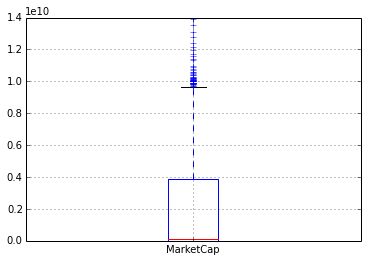
\includegraphics[width=1\linewidth]
    {gfx/market-cap-boxplot}}
  \caption{Market Capitalization Boxplot}
  \label{fig:market-cap-boxplot}
\end{figure}

\clearpage
%----------------------------------------------------------------------

\subsection{Market Price}
\label{sec:market-price}

\begin{figure}[bth]
  \myfloatalign
  {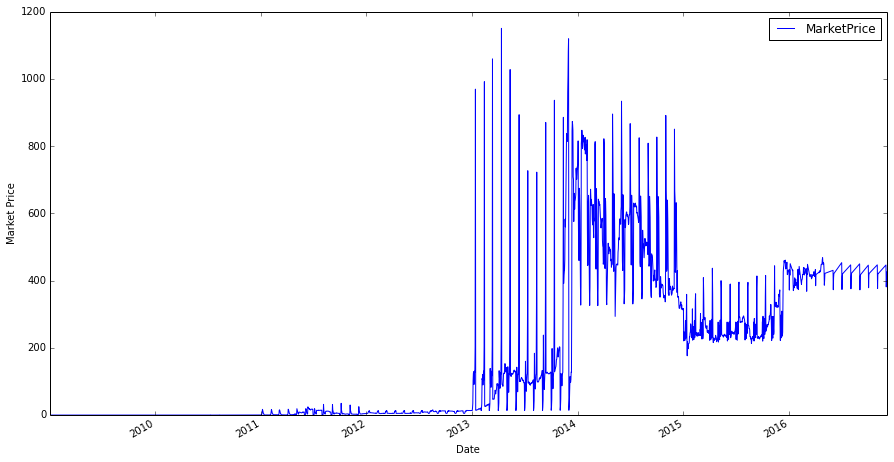
\includegraphics[width=1\linewidth]
    {gfx/market-price-over-time}}
  \caption{Market Price Over Time}
  \label{fig:market-price-over-time}
\end{figure}

Average USD market price across major Bitcoin exchanges.
\autoref{fig:market-price-over-time} is identical to the one in
\autoref{fig:market-cap-over-time} except for the scale. The same
events that produced the market capitalization fluctuation apply to
the market price. Added to that, the average market price across mayor
Bitcoin exchange operators is a variable very closely related to the
market capitalization of Bitcoin.

Is important to note how volatile is the Bitcoin average price,
ranging from nearly $0$ USD to $1100$ USD in just a year, and now, in
2016 fluctuating in a range bigger than $10$ USD on average. This
fluctuations, if predicted, can be very profitable for the trader. 

The data-set comprises one real number data point each day, at
18:15:05, spanning from 03/01/2009 to 03/05/2016.

\begin{table}
  \myfloatalign
  %\small
  \begin{tabularx}{\textwidth}{XX} 
    \toprule
    \tableheadline{Measure} & \tableheadline{Value} \\
    \midrule 
    count  & $2678$       \\
    mean   & $155.924369$ \\
    median & $12.37856$   \\
    std    & $218.563332$ \\
    min    & $0$          \\
    $25$\% & $0.20925$    \\
    $50$\% & $12.378560$  \\
    $75$\% & $271.335$    \\
    max    & $1151$       \\
    \bottomrule
  \end{tabularx}
  \caption{Statistical values for \textit{Market Price}}
  \label{tab:market-price}
\end{table}

\begin{figure}[bth]
  \myfloatalign
  {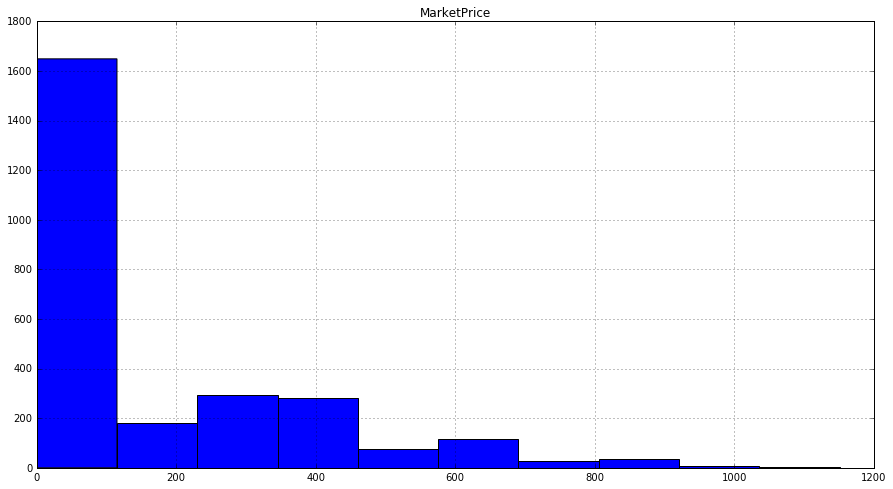
\includegraphics[width=1\linewidth]
    {gfx/market-price-histogram}}
  \caption{Market Price Histogram}
  \label{fig:market-price-histogram}
\end{figure}

\begin{figure}[bth]
  \myfloatalign
  {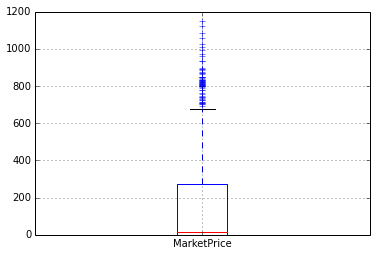
\includegraphics[width=1\linewidth]
    {gfx/market-price-boxplot}}
  \caption{Market Price Boxplot}
  \label{fig:market-price-boxplot}
\end{figure}

\clearpage
%----------------------------------------------------------------------

\subsection{Median Confirmation Time}
\label{sec:median-confirmation-time}

\begin{figure}[bth]
  \myfloatalign
  {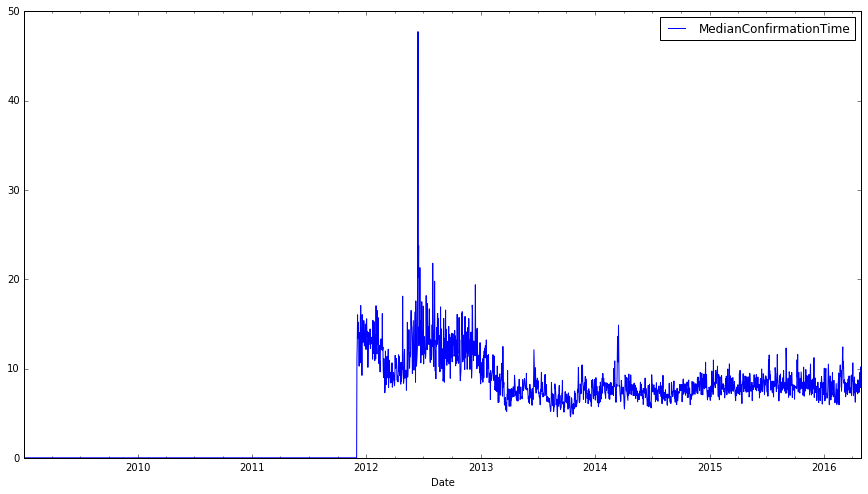
\includegraphics[width=1\linewidth]
    {gfx/median-confirmation-time-over-time}}
  \caption{Median Confirmation Time Over Time}
  \label{fig:median-confirmation-time-over-time}
\end{figure}

The median time for a transaction to be accepted into a mined block
and added to the public ledger (note: only includes transactions with
miner fees). Until the end of 2011, the confirmation time is
negligible. There is an important event that can be related to the
growth of the median confirmation time, and that is the largest
Bitcoin fee in a single transaction, in December 12, 171 Bitcoins was
paids as fee in block 157235.

If we look at \autoref{fig:median-confirmation-time-over-time} there
is a peak in mid 2012, that can coincide with the increase in number
of transactions seen in
\autoref{fig:n-transactions-multiple-over-time}. After that even
though the number of transactions is growing, there is also in
increment in the hash rate, so the number of transactions can be
included in blocks thanks to the amount of miners and their processing
power.

 One real number data point each day, at 18:15:05,
spanning from 03/01/2009 to 03/05/2016.

\begin{table}
  \myfloatalign
  %\small
  \begin{tabularx}{\textwidth}{XX} 
    \toprule
    \tableheadline{Measure} & \tableheadline{Value} \\
    \midrule 
    count  & $2678$      \\
    mean   & $5.38554$   \\
    median & $6.975$     \\
    std    & $4.859709$  \\
    min    & $0$         \\
    $25$\% & $0$         \\
    $50$\% & $6.975$     \\
    $75$\% & $8.5$       \\
    max    & $47.733333$ \\
    \bottomrule
  \end{tabularx}
  \caption{Statistical values for 
    \textit{Median Confirmation Time}}
  \label{tab:median-confirmation-time}
\end{table}

\begin{figure}[bth]
  \myfloatalign
  {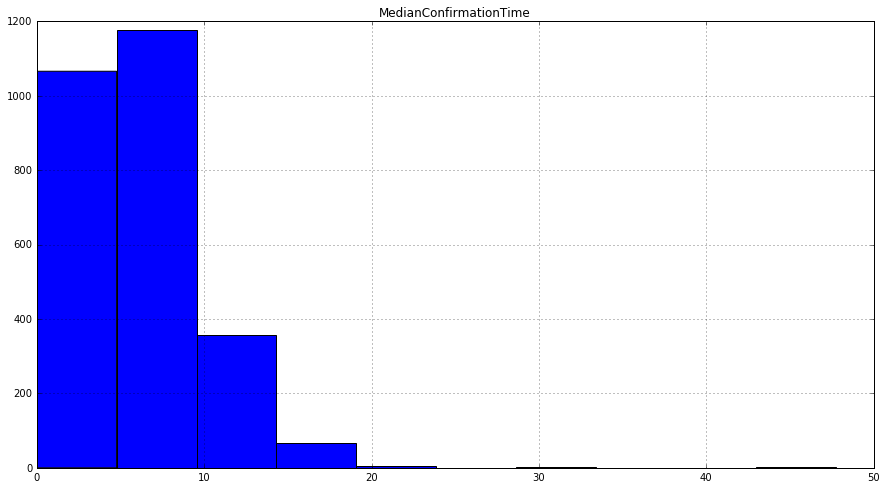
\includegraphics[width=1\linewidth]
    {gfx/median-confirmation-time-histogram}}
  \caption{Median Confirmation Time Histogram}
  \label{fig:median-confirmation-time-histogram}
\end{figure}

\begin{figure}[bth]
  \myfloatalign
  {\includegraphics[width=1\linewidth]
    {gfx/median-confirmation-time-boxplot}}
  \caption{Median Confirmation Time Boxplot}
  \label{fig:median-confirmation-time-boxplot}
\end{figure}

\clearpage
%----------------------------------------------------------------------

\subsection{Miners Revenue}
\label{sec:miners-revenue}

\begin{figure}[bth]
  \myfloatalign
  {\includegraphics[width=1\linewidth]
    {gfx/miners-revenue-over-time}}
  \caption{Miners Revenue Over Time}
  \label{fig:miners-revenue-over-time}
\end{figure}

Total value of coinbase block rewards and transaction fees paid to
miners, expressed in USD. To understand the rewards and fees, we
include this quote, extracted the 1st of June of 2016 from
\href{https://en.bitcoin.it/wiki/Mining}{https://en.bitcoin.it/wiki/Mining}:

\textit{``When a block is discovered, the discoverer may award
  themselves a certain number of bitcoins, which is agreed-upon by
  everyone in the network. Currently this bounty is 25 bitcoins; this
  value will halve every 210,000 blocks. [...]. } 

\textit{Additionally, the miner is awarded the fees paid by users
  sending transactions. The fee is an incentive for the miner to
  include the transaction in their block. In the future, as the number
  of new bitcoins miners are allowed to create in each block dwindles,
  the fees will make up a much more important percentage of mining
  income.''}

Taking the previous quote into consideration, we know that the miner
reward is fixed, so its fluctuation will depend upon the price of the
Bitcoin itself, therefore the resemblance between miners revenue
(\autoref{fig:miners-revenue-over-time}) and Bitcoin price
(\autoref{fig:market-price-over-time}).

In 2016, the transaction fees represent a very small amount of the
BTCs of the miners revenue. We can see in
\autoref{tab:cost-per-transaction} that the average transaction has a
value of $9.727391$. On the other hand, the average number of
transactions per block $306.632248$. Thus the expected revenue due to
fees of a single miner is $9.727391 \times 306.632248 = $
$2982.7317695049683$ USD.

If we analyze the revenue thanks to the reward of discovering a block
we have that the average market price of the
Bitcoin(\autoref{tab:market-price}) is $155.924369$ USD and the reward
is $25$ BTC per block discovered, that makes an amount of $155.924369
\times 25 = 3898.109225$ USD per block discovered. Added to that, we
have to keep in mind that, as of June the $2^{nd}$, the current price
of Bitcoin is $536.99$ USD, which makes the rewards value increase to
$536.99 \times 25 = 13424.75$ USD per blocked discovered. We can
conclude that nowadays, the main source of revenues for miners is the
block discovery, but in the future, as it goes getting harder to
discover blocks, the fees will start to be an important source of
income for miners. 

This data-set comprises one real number data point each day, at
18:15:05, spanning from 03/01/2009 to 03/05/2016.

\begin{table}
  \myfloatalign
  %\small
  \begin{tabularx}{\textwidth}{XX} 
    \toprule
    \tableheadline{Measure} & \tableheadline{Value} \\
    \midrule 
    count  & $2678.000000$    \\
    mean   & $638331.424709$  \\
    median & $85611.64705$    \\
    std    & $911565.967412$  \\
    min    & $0.000000$       \\
    $25$\% & $1895.375000$    \\
    $50$\% & $85611.647050$   \\
    $75$\% & $1023087.365000$ \\
    max    & $5117346.000000$ \\
    \bottomrule
  \end{tabularx}
  \caption{Statistical values for \textit{Miners Revenue}}
  \label{tab:miners-revenue}
\end{table}

\begin{figure}[bth]
  \myfloatalign
  {\includegraphics[width=1\linewidth]
    {gfx/miners-revenue-histogram}}
  \caption{Miners Revenue Histogram}
  \label{fig:miners-revenue-histogram}
\end{figure}

\begin{figure}[bth]
  \myfloatalign
  {\includegraphics[width=1\linewidth]
    {gfx/miners-revenue-boxplot}}
  \caption{Miners Revenue Boxplot}
  \label{fig:miners-revenue-boxplot}
\end{figure}

\clearpage
%----------------------------------------------------------------------

\subsection{Network Deficit}
\label{sec:network-deficit}

\begin{figure}[bth]
  \myfloatalign
  {\includegraphics[width=1\linewidth]
    {gfx/network-deficit-over-time}}
  \caption{Network Deficit Over Time}
  \label{fig:network-deficit-over-time}
\end{figure}

Shows difference between transaction fees and cost of Bitcoin mining
in USD. This definition, given by
\href{https://blockchain.info/charts}{BlockChain.info} can be a little
bit misleading, because it's not clear what the \textit{cost of
  Bitcoin mining} means. After some research, we found in
\href{http://bitcoin.stackexchange.com/questions/10230/how-is-network-deficit-calculated}{StackExchange}
that the cost of Bitcoin mining is the reward from Bitcoin mining. So
the network deficit, is the difference between transaction fees and
reward for mining. There is a lot of discussion about what this
variable represents, and how to interpret it. For example:

``\textit{So at the current rate of 1 tps, the average transaction fee
  would need to rise to \$5 worth of BTC to keep mining at its current
  economic strength. This would drastically reduce write access to
  Bitcoin, and might not even be achievable due to consumer choice
  (growing preference among potential adoptees for market alternatives
  like traditional finance, alt-blockchains, etc as the average tx fee
  increases).}

\textit{While decentralization has been the main focus of the block
  size debate, hashrate (mining revenues) and accessibility (cost of
  transaction) are also important metrics of network utility and
  health, and should be taken into consideration.}

\textit{The lower the maximum transaction throughput, the more
  expensive transactions need to be to maintain current mining
  revenues. The optimal block size limit will strike the right balance
  between mining decentralization, miner revenue, and write
  accessibility, and not exclude any of these factors in its focus.}''

What we see in \autoref{fig:network-deficit-over-time} is that as
mentioned before in \autoref{sec:miners-revenue}, the revenues of
miners are mostly due to the rewards of block discovery instead of the
fees produced in transactions. This can be interpreted as a network
inmaturity, because miners, which are the main supporters of the
Bitcoin network, rely mostly on the Bitcoin inflation to make profit,
instead of the transactions and associated fees.

It's easy to see the relationship between the network deficit and the
Bitcoin market price by noticing that
\autoref{fig:network-deficit-over-time} and
\autoref{fig:market-price-over-time} are nearly simetrical in the X
axis. So, the higher the price of bitcoin, the higher is the deficit
(though is represented in negative numbers).

This data-set comprises one real number data point each day, at
18:15:05, spanning from 03/01/2009 to 03/05/2016.


\begin{table}
  \myfloatalign
  %\small
  \begin{tabularx}{\textwidth}{XX} 
    \toprule
    \tableheadline{Measure} & \tableheadline{Value} \\
    \midrule 
    count  & $2678$ \\
    mean   & -$631395.059680$ \\
    median & -$84958.600143$ \\
    std    & $903713.147531$ \\
    min    & -$5068845.988395$ \\
    $25$\% & -$1009464.098582$ \\
    $50$\% & -$84958.600143$ \\
    $75$\% & -$1895.354052$ \\
    max    & $0$ \\
    \bottomrule
  \end{tabularx}
  \caption{Statistical values for \textit{Network Deficit}}
  \label{tab:network-deficit}
\end{table}

\begin{figure}[bth]
  \myfloatalign
  {\includegraphics[width=1\linewidth]
    {gfx/network-deficit-histogram}}
  \caption{Network Deficit Histogram}
  \label{fig:network-deficit-histogram}
\end{figure}

\begin{figure}[bth]
  \myfloatalign
  {\includegraphics[width=1\linewidth]
    {gfx/network-deficit-boxplot}}
  \caption{Network Deficit Boxplot}
  \label{fig:network-deficit-boxplot}
\end{figure}

\clearpage
%----------------------------------------------------------------------

\subsection{Number of Transactions}
\label{sec:n-transactions-multiple}

\begin{figure}[bth]
  \myfloatalign
  {\includegraphics[width=1\linewidth]
    {gfx/n-transactions-multiple-over-time}}
  \caption{Number of Transactions Over Time}
  \label{fig:n-transactions-multiple-over-time}
\end{figure}

Here we analyze a compound set of variables: number of transactions,
number of transactions excluding chains longer than 10, 100, 1000 and
10000, and number of transactions excluding the 100 most popular
addresses. 

The number of transactions is defined as ``\textit{The number of daily
  confirmed Bitcoin transactions}''. As for long chains, we include a
quote from
\href{http://www.ofnumbers.com/2015/01/22/slicing-data-what-comprises-blockchain-transactions/}{Tim
  Swanson} that explains the origin of the term and why can be useful:
``\textit{questions have arisen over a series of what some call “long
  chains.” Last month several commentators on a popular thread on
  Hacker News identified thousands of small transactions originating
  from a single source. The source was continually sending
  transactions and paid transaction fees for each of them. The reason
  this struck many as odd as a rational actor would simply bundle the
  transactions together to save on transaction fees.}

\textit{ While there are likely different motivations for doing so,
  one reason for why this was occurring was that the originating
  source was attempting to delink or otherwise mix and tumble coins to
  make it difficult to “dox” or identify the originating source. But
  it could also be a faucet and at one point even pools paid out
  miners using chained transactions, perhaps some still do.}''


The number of transactions represented in blue color in
\autoref{fig:n-transactions-multiple-over-time} show a moderated
growth compared to that of the market price or market capitalization.
That may be because this variable doesn't depend on the inflation of
the Bitcoin, and there aren't exagerated fluctuation. We see that even
the price of the Bitcoin is not at its peak in 2016, the number of
transactions are in the higher point so far in the Bitcoin history.
It's also possible to see the relatioship between the different curves
excluding ``long chains'', where as the ``long chains'' are removed
the number of transactions decrease, although the tendency is similar.

Regarding \textit{number of transactions excluding popular}, is useful
to show whether there is a dependecy of a small number of actors in
the Bitcoin network. What we see in
\autoref{fig:n-transactions-multiple-over-time} is that,
\textit{number of transactions excluding popular} in yellow, is
growing independent from the 100 most popular addresses. While until
2014 this addresses added a substantial amount of transactions to the
overall count, from that point on, the count between the total
transactions and \textit{number of transactions excluding popular} is
similar.

This data-set comprises six integer data point each day, at 18:15:05,
spanning from 03/01/2009 to 03/05/2016.

\begin{table}
  \myfloatalign
  \tiny
  \begin{tabularx}{\textwidth}{XXXXXXX} 
    \toprule
    \tableheadline{Measure} &
    \tableheadline{NumTransactions} &
    \tableheadline{Excluding10} &
    \tableheadline{Excluding100} &
    \tableheadline{Excluding1000} &
    \tableheadline{Excluding10000} &
    \tableheadline{ExcludingPopular} \\
    \midrule                                                                                     
    count  & $2678$         & $2678$         & $2678$         & $2678$         & $2678$         & $2678$         \\
    mean   & $47255.265497$ & $15589.57879$  & $26050.881255$ & $32665.966019$ & $39117.017177$ & $40400.536968$ \\
    median & $31214$        & $7115$         & $12810$        & $16915$        & $22558$        & $12597.5$      \\
    std    & $56769.848304$ & $20367.504877$ & $32164.862369$ & $40035.066692$ & $46391.775343$ & $55357.260528$ \\
    min    & $0$            & $0$            & $0$            & $0$            & $0$            & $0$            \\
    $25$\  & $501.5$        & $337$          & $426.25$       & $486.25$       & $501.5$        & $501.5$        \\
    $50$\  & $31214$        & $7115$         & $12810$        & $16915$        & $22558$        & $12597.5$      \\
    $75$\  & $69853$        & $23695.5$      & $39936.75$     & $50210.75$     & $61130$        & $63434.25$     \\
    max    & $276448$       & $157002$       & $187035$       & $206184$       & $227830$       & $262461$       \\
    \bottomrule
  \end{tabularx}
  \caption{Statistical values for \textit{Number of Transactions}}
  \label{tab:n-transactions-multiple}
\end{table}

\begin{figure}[bth]
  \myfloatalign
  {\includegraphics[width=1\linewidth]
    {gfx/n-transactions-multiple-histogram}}
  \caption{Number of Transactions Histogram}
  \label{fig:n-transactions-multiple-histogram}
\end{figure}

\begin{figure}[bth]
  \myfloatalign
  {\includegraphics[width=1\linewidth]
    {gfx/n-transactions-multiple-boxplot}}
  \caption{Number of Transactions Boxplot}
  \label{fig:n-transactions-multiple-boxplot}
\end{figure}

\clearpage
%----------------------------------------------------------------------

\subsection{Number of Transactions Per Block}
\label{sec:n-transactions-per-block}

\begin{figure}[bth]
  \myfloatalign
  {\includegraphics[width=1\linewidth]
    {gfx/n-transactions-per-block-over-time}}
  \caption{Number of Transactions Per Block
    Over Time}
  \label{fig:n-transactions-per-block-over-time}
\end{figure}

This variable represents the average number of transactions per block.
The way transactions are added to the Bitcoin network is by adding
them to a block. This operation is done by miners, that receive a fee
(that can be zero) to do this operation. As mentioned before, today,
miners revenue are due mostly to the discovery of new blocks instead
of fees, nonetheless fees is another source of income. A miner can
choose not to include transactions in the mined blocks, and that would
go against the healthy growth of the Bitcoin network. Fortunately,
\autoref{fig:n-transactions-per-block-over-time} shows that the amount
of transactions per block is increasing, this way Bitcoin networks can
keep growing relying in miners to process transactions. On top of
that, the average amount of transactions per block since mid 2015 is
greater than $1000$, given that the average cost per transaction is
$9.727391$ which gives an average revenue of $9727.391$ USD per block
for miner for this period.

This data-set comprises one integer data point each day, at 18:15:05,
spanning from 03/01/2009 to 28/04/2016.

\begin{table}
  \myfloatalign
  %\small
  \begin{tabularx}{\textwidth}{XX} 
    \toprule
    \tableheadline{Measure} & \tableheadline{Value} \\
    \midrule 
    count  & $2673$ \\
    mean   & $306.632248$  \\
    median & $205$         \\
    std    & $377.986965$  \\
    min    & $1$    \\
    $25$\% & $2$    \\
    $50$\% & $205$  \\
    $75$\% & $435$  \\
    max    & $2036$ \\
    \bottomrule
  \end{tabularx}
  \caption{Statistical values for \textit{Number of Transactions 
      Per Block}}
  \label{tab:n-transactions-per-block}
\end{table}

\begin{figure}[bth]
  \myfloatalign
  {\includegraphics[width=1\linewidth]
    {gfx/n-transactions-per-block-histogram}}
  \caption{Number of Transactions Per Block
    Histogram}
  \label{fig:n-transactions-per-block-histogram}
\end{figure}

\begin{figure}[bth]
  \myfloatalign
  {\includegraphics[width=1\linewidth]
    {gfx/n-transactions-per-block-boxplot}}
  \caption{Number of Transactions Per Block
    Boxplot}
  \label{fig:n-transactions-per-block-boxplot}
\end{figure}

\clearpage
%---------------------------------------------------------------------- 

\subsection{Number of Total Transactions}
\label{sec:n-transactions-total}

\begin{figure}[bth]
  \myfloatalign
  {\includegraphics[width=1\linewidth]
    {gfx/n-transactions-total-over-time}}
  \caption{Number of Total Transactions
    Over Time}
  \label{fig:n-transactions-total-over-time}
\end{figure}


Total number of transactions data in
\autoref{fig:n-transactions-total-over-time} show that the growth is
exponential. It can be seen in
\autoref{fig:n-transactions-multiple-over-time} that the number of
transactions per day is increasing, from that we can assume that the
growth of accumulated number of transactions over time is going to
increase in a nearly exponential way.

This data-set comprises one integer data point each day, at 18:15:05,
spanning from 03/01/2009 to 03/05/2016.

\begin{table}
  \myfloatalign
  %\small
  \begin{tabularx}{\textwidth}{XX} 
    \toprule
    \tableheadline{Measure} & \tableheadline{Value} \\
    \midrule 
    count  & $2.678000e+03$ \\
    mean   & $2.491078e+07$ \\
    median & $6685067$      \\
    std    & $3.308262e+07$ \\
    min    & $1$ \\
    $25$\% & $1.384448e+05$ \\
    $50$\% & $6.685067e+06$ \\
    $75$\% & $4.191287e+07$ \\
    max    & $1.265496e+08$ \\
    \bottomrule
  \end{tabularx}
  \caption{Statistical values for \textit{Number of Total
      Transactions}}
  \label{tab:n-transactions-total}
\end{table}

\begin{figure}[bth]
  \myfloatalign
  {\includegraphics[width=1\linewidth]
    {gfx/n-transactions-total-histogram}}
  \caption{Number of Total Transactions
    Histogram}
  \label{fig:n-transactions-total-histogram}
\end{figure}

\begin{figure}[bth]
  \myfloatalign
  {\includegraphics[width=1\linewidth]
    {gfx/n-transactions-total-boxplot}}
  \caption{Number of Total Transactions
    Boxplot}
  \label{fig:n-transactions-total-boxplot}
\end{figure}

\clearpage
%---------------------------------------------------------------------- 

\subsection{Number of Unique Addresses}
\label{sec:n-unique-addresses}

\begin{figure}[bth]
  \myfloatalign
  {\includegraphics[width=1\linewidth]
    {gfx/n-unique-addresses-over-time}}
  \caption{Number of Unique Addresses
    Over Time}
  \label{fig:n-unique-addresses-over-time}
\end{figure}

The total number of unique addresses used on the Bitcoin blockchain. A
unique adress, as defined by
\href{https://en.bitcoin.it/wiki/Address}{Bitcoin.it}: ``\textit{A
  Bitcoin address, or simply address, is an identifier of 26-35
  alphanumeric characters, beginning with the number 1 or 3, that
  represents a possible destination for a bitcoin payment.}'' This
variable is closely related to the number of transactions made in the
network. When compared,
\autoref{fig:n-transactions-multiple-over-time} and
\autoref{fig:n-unique-addresses-over-time} show a resemblance not only
in the events that produce the local maximums but also in the growth.

This data-set comprises one integer data point each day, at 18:15:05,
spanning from 03/01/2009 to 03/05/2016.

\begin{table}
  \myfloatalign
  %\small
  \begin{tabularx}{\textwidth}{XX} 
    \toprule
    \tableheadline{Measure} & \tableheadline{Value} \\
    \midrule 
    count  & $2678$          \\
    mean   & $86921.616878$  \\
    median & $29205.5$       \\
    std    & $112219.880994$ \\
    min    & $0$             \\
    $25$\% & $609.25$        \\
    $50$\% & $29205.5$       \\
    $75$\% & $152308.5$      \\
    max    & $483756$        \\
    \bottomrule
  \end{tabularx}
  \caption{Statistical values for \textit{Number of Unique Addresses}}
  \label{tab:n-unique-addresses}
\end{table}

\begin{figure}[bth]
  \myfloatalign
  {\includegraphics[width=1\linewidth]
    {gfx/n-unique-addresses-histogram}}
  \caption{Number of Unique Addresses
    Histogram}
  \label{fig:n-unique-addresses-histogram}
\end{figure}

\begin{figure}[bth]
  \myfloatalign
  {\includegraphics[width=1\linewidth]
    {gfx/n-unique-addresses-boxplot}}
  \caption{Number of Unique Addresses
    Boxplot}
  \label{fig:n-unique-addresses-boxplot}
\end{figure}

\clearpage
%--------------------------------------------------------------------- 

\subsection{Output Volume}
\label{sec:output-volume}

\begin{figure}[bth]
  \myfloatalign
  {\includegraphics[width=1\linewidth]
    {gfx/output-volume-over-time}}
  \caption{Output Volume
    Over Time}
  \label{fig:output-volume-over-time}
\end{figure}

The total value of all transaction outputs per day (includes coins
returned to the sender as change). It's easier to understand to
meaning of output and change in the bitcoin world with an explanation
given by a user nicknamed \textit{DeathAndTaxes} in
\href{https://bitcointalk.org/index.php?topic=99593.0}{Bitcointalk.org}:

``\textit{Bitcoin can only create transactions by using as the input
  an ENTIRE prior unspent output. The most important thing to realize
  is that Bitcoin tx have inputs and outputs. The "value" of your
  wallet is an abstraction. It is simply your client (software which
  analyzes the wallet) taking a SUM of all the unspent outputs which
  you have private keys for. The input of a tx is the output of a
  PRIOR tx. You can only use unspent outputs in a new tx. Once they
  are part of a tx they can never be used again ("spent").}

\textit{Say you I send you 50 BTC (for simplicity lets assume this is
  compromised of a single 50 BTC output). No matter how you spend that
  the input for the tx will be 50 BTC.}

\textit{Want to spend 20 BTC? Input: 50 BTC Output: 20 BTC + 30 BTC
  "change" back to an address you control. Want to spend 1 BTC? Input:
  50 BTC Output: 1 BTC + 49 BTC "change" back to an address you
  control.}''

Output can be due to three circumstances, large amout of transactions,
transactions of big amount of Bitcoins, and big amount of change
returned to sender. The peak of 2013 is clearly due to change received
by sender as \textit{DeathAndTaxes} explains: ``\textit{In the early
  days of Bitcoin there really was nothing to "spend" it on so most tx
  tended to be accumulation. This resulted in most addresses having
  very large unspent outputs. As people started "breaking" up those
  unspent outputs in tx involving smaller amounts most of the volume
  WAS change.}''

This data-set comprises one real number data point each day, at
18:15:05, spanning from 03/01/2009 to 03/05/2016.

\begin{table}
  \myfloatalign
  %\small
  \begin{tabularx}{\textwidth}{XX} 
    \toprule
    \tableheadline{Measure} & \tableheadline{Value} \\
    \midrule 
    count  & $2679$            \\
    mean   & $1134859.87078$   \\
    median & $661019.796765$   \\
    std    & $2333431.889695$  \\
    min    & $0$               \\
    $25$\% & $73233.013445$    \\
    $50$\% & $661019.796765$   \\
    $75$\% & $1286432.155226$  \\
    max    & $45992222.558034$ \\
    \bottomrule
  \end{tabularx}
  \caption{Statistical values for \textit{Output Volume}}
  \label{tab:output-volume}
\end{table}

\begin{figure}[bth]
  \myfloatalign
  {\includegraphics[width=1\linewidth]
    {gfx/output-volume-histogram}}
  \caption{Output Volume
    Histogram}
  \label{fig:output-volume-histogram}
\end{figure}

\begin{figure}[bth]
  \myfloatalign
  {\includegraphics[width=1\linewidth]
    {gfx/output-volume-boxplot}}
  \caption{Output Volume
    Boxplot}
  \label{fig:output-volume-boxplot}
\end{figure}

\clearpage
%--------------------------------------------------------------------- 

\subsection{Standard Output Volume Poors 500}
\label{sec:standard-and-poors-500}

\begin{figure}[bth]
  \myfloatalign
  {\includegraphics[width=1\linewidth]
    {gfx/standard-and-poors-500-over-time}}
  \caption{Standard Output Volume Poors 500
    Over Time}
  \label{fig:standard-and-poors-500-over-time}
\end{figure}

Six real data point entry each day, spanning from 03/01/1950 to
09/05/2016. The variable names are \textit{Open}, \textit{High},
\textit{Low}, \textit{Close}, \textit{Volume}, \textit{Adj} and
\textit{Close}, representing different characteristics of the index
price.

From the Wikipedia: ``\textit{The Standard \& Poor's 500, often
  abbreviated as the S\&P 500, or just "the S\&P", is an American
  stock market index based on the market capitalizations of 500 large
  companies having common stock listed on the NYSE or NASDAQ. The S\&P
  500 index components and their weightings are determined by S\&P Dow
  Jones Indices. It differs from other U.S. stock market indices, such
  as the Dow Jones Industrial Average or the Nasdaq Composite index,
  because of its diverse constituency and weighting methodology. It is
  one of the most commonly followed equity indices, and many consider
  it one of the best representations of the U.S. stock market, and a
  bellwether for the U.S. economy. The National Bureau of Economic
  Research has classified common stocks as a leading indicator of
  business cycles.}''

\begin{table}
  \myfloatalign
  \tiny
  \begin{tabularx}{\textwidth}{XXXXXXX} 
    \toprule
    \tableheadline{Measure} & \tableheadline{Open} &
    \tableheadline{High} & \tableheadline{Low} & \tableheadline{Close}
    & \tableheadline{Volume} & \tableheadline{Adj Close}\\
    \midrule 
    count  & $16695$       & $16695$       & $16695$       & $16695$       & $1.669500e+04$ & $16695$       \\
    mean   & $492.103240$  & $495.207861$  & $488.827423$  & $492.221084$  & $8.157494e+08$ & $492.221084$  \\
    median & $150.910004$  & $151.619995$  & $150.240005$  & $151.039993$  & $75180000$     & $151.039993$  \\
    std    & $566.001594$  & $569.347411$  & $562.382420$  & $566.107954$  & $1.478957e+09$ & $566.107954$  \\
    min    & $16.660000$   & $16.660000$   & $16.660000$   & $16.660000$   & $6.800000e+05$ & $16.660000$   \\
    $25$\% & $84.099998$   & $84.765000$   & $83.459999$   & $84.099998$   & $7.805000e+06$ & $84.099998$   \\
    $50$\% & $150.910004$  & $151.619995$  & $150.240005$  & $151.039993$  & $7.518000e+07$ & $151.039993$  \\
    $75$\% & $974.309998$  & $983.190002$  & $964.844971$  & $974.904999$  & $8.428500e+08$ & $974.904999$  \\
    max    & $2130.360107$ & $2134.719971$ & $2126.060059$ & $2130.820068$ & $1.145623e+10$ & $2130.820068$ \\
    \bottomrule
  \end{tabularx}
  \caption{Statistical values for \textit{Standard Output Volume Poors 500}}
  \label{tab:standard-and-poors-500}
\end{table}

\begin{figure}[bth]
  \myfloatalign
  {\includegraphics[width=1\linewidth]
    {gfx/standard-and-poors-500-histogram}}
  \caption{Standard Output Volume Poors 500
    Histogram}
  \label{fig:standard-and-poors-500-histogram}
\end{figure}

\begin{figure}[bth]
  \myfloatalign
  {\includegraphics[width=1\linewidth]
    {gfx/standard-and-poors-500-boxplot}}
  \caption{Standard Output Volume Poors 500
    Boxplot}
  \label{fig:standard-and-poors-500-boxplot}
\end{figure}

Due to the difference in scale of the variable \textit{Volume}
compared to the rest of variables it's not possible to see their
boxplots in \autoref{fig:standard-and-poors-500-boxplot}. We need
another boxplot, seen in
\autoref{fig:standard-and-poors-500-rest-boxplot}, for the rest of the
variables to be seen clearly.

\begin{figure}[bth]
  \myfloatalign
  {\includegraphics[width=1\linewidth]
    {gfx/standard-and-poors-500-rest-boxplot}}
  \caption{Standard Output Volume Poors 500
    Rest of Variables Boxplot}
  \label{fig:standard-and-poors-500-rest-boxplot}
\end{figure}

\clearpage
%--------------------------------------------------------------------- 

\subsection{Total Bitcoins}
\label{sec:total-bitcoins}

\begin{figure}[bth]
  \myfloatalign
  {\includegraphics[width=1\linewidth]
    {gfx/total-bitcoins-over-time}}
  \caption{Total Bitcoins
    Over Time}
  \label{fig:total-bitcoins-over-time}
\end{figure}

The total number of bitcoins that have already been mined; in other
words, the current supply of bitcoins on the network. One integer data
point each day, at 18:15:05, spanning from 03/01/2009 to 03/05/2016.

\begin{table}
  \myfloatalign
  %\small
  \begin{tabularx}{\textwidth}{XX} 
    \toprule
    \tableheadline{Measure} & \tableheadline{Value} \\
    \midrule 
    count  & $2.678000e+03$ \\
    mean   & $8.723580e+06$ \\
    median & $9849250.0$    \\
    std    & $4.819287e+06$ \\
    min    & $5.000000e+01$ \\
    $25$\% & $4.472438e+06$ \\
    $50$\% & $9.849250e+06$ \\
    $75$\% & $1.297915e+07$ \\
    max    & $1.550142e+07$ \\
    \bottomrule
  \end{tabularx}
  \caption{Statistical values for \textit{Total Bitcoins}}
  \label{tab:total-bitcoins}
\end{table}

\begin{figure}[bth]
  \myfloatalign
  {\includegraphics[width=1\linewidth]
    {gfx/total-bitcoins-histogram}}
  \caption{Total Bitcoins
    Histogram}
  \label{fig:total-bitcoins-histogram}
\end{figure}

\begin{figure}[bth]
  \myfloatalign
  {\includegraphics[width=1\linewidth]
    {gfx/total-bitcoins-boxplot}}
  \caption{Total Bitcoins
    Boxplot}
  \label{fig:total-bitcoins-boxplot}
\end{figure}

\clearpage
%--------------------------------------------------------------------- 

\subsection{Trade Volume}
\label{sec:trade-volume}

\begin{figure}[bth]
  \myfloatalign
  {\includegraphics[width=1\linewidth]
    {gfx/trade-volume-over-time}}
  \caption{Trade Volume
    Over Time}
  \label{fig:trade-volume-over-time}
\end{figure}

The total USD value of trading volume on major bitcoin exchanges. One
real number data point each day, at 18:15:05, spanning from 03/01/2009
to 03/05/2016.

\begin{table}
  \myfloatalign
  %\small
  \begin{tabularx}{\textwidth}{XX} 
    \toprule
    \tableheadline{Measure} & \tableheadline{Value} \\
    \midrule 
    count  & $2.678000e+03$  \\
    mean   & $2.768062e+06$  \\
    median & $529334.610415$ \\
    std    & $5.819032e+06$  \\
    min    & $0.000000e+00$  \\
    $25$\% & $1.341996e+03$  \\
    $50$\% & $5.293346e+05$  \\
    $75$\% & $3.014521e+06$  \\
    max    & $7.205049e+07$  \\
    \bottomrule
  \end{tabularx}
  \caption{Statistical values for \textit{Trade Volume}}
  \label{tab:trade-volume}
\end{table}

\begin{figure}[bth]
  \myfloatalign
  {\includegraphics[width=1\linewidth]
    {gfx/trade-volume-histogram}}
  \caption{Trade Volume
    Histogram}
  \label{fig:trade-volume-histogram}
\end{figure}

\begin{figure}[bth]
  \myfloatalign
  {\includegraphics[width=1\linewidth]
    {gfx/trade-volume-boxplot}}
  \caption{Trade Volume
    Boxplot}
  \label{fig:trade-volume-boxplot}
\end{figure}

\clearpage
%--------------------------------------------------------------------- 

\subsection{Transaction Fees}
\label{sec:transaction-fees}

\begin{figure}[bth]
  \myfloatalign
  {\includegraphics[width=1\linewidth]
    {gfx/transaction-fees-over-time}}
  \caption{Transaction Fees
    Over Time}
  \label{fig:transaction-fees-over-time}
\end{figure}

The total value of all transaction fees paid to miners (not including
the coinbase value of block rewards) in BTC. One real number data
point each day, at 18:15:05, spanning from 03/01/2009 to 03/05/2016.

\begin{table}
  \myfloatalign
  %\small
  \begin{tabularx}{\textwidth}{XX} 
    \toprule
    \tableheadline{Measure} & \tableheadline{Value} \\
    \midrule 
    count  & $2678.000000$ \\
    mean   & $16.273161$   \\
    median & $12.23832$    \\
    std    & $20.839539$   \\
    min    & $0.000000$    \\
    $25$\% & $0.070599$    \\
    $50$\% & $12.238320$   \\
    $75$\% & $25.172616$   \\
    max    & $336.577055$  \\
    \bottomrule
  \end{tabularx}
  \caption{Statistical values for \textit{Transaction Fees}}
  \label{tab:transaction-fees}
\end{table}

\begin{figure}[bth]
  \myfloatalign
  {\includegraphics[width=1\linewidth]
    {gfx/transaction-fees-histogram}}
  \caption{Transaction Fees
    Histogram}
  \label{fig:transaction-fees-histogram}
\end{figure}

\begin{figure}[bth]
  \myfloatalign
  {\includegraphics[width=1\linewidth]
    {gfx/transaction-fees-boxplot}}
  \caption{Transaction Fees
    Boxplot}
  \label{fig:transaction-fees-boxplot}
\end{figure}

\clearpage
%--------------------------------------------------------------------- 

\subsection{Transaction Fees USD}
\label{sec:transaction-fees-usd}

\begin{figure}[bth]
  \myfloatalign
  {\includegraphics[width=1\linewidth]
    {gfx/transaction-fees-usd-over-time}}
  \caption{Transaction Fees USD
    Over Time}
  \label{fig:transaction-fees-usd-over-time}
\end{figure}

The total value of all transaction fees paid to miners (not including
the coinbase value of block rewards) in USD. One real number data
point each day, at 18:15:05, spanning from 03/01/2009 to 03/05/2016.

\begin{table}
  \myfloatalign
  %\small
  \begin{tabularx}{\textwidth}{XX} 
    \toprule
    \tableheadline{Measure} & \tableheadline{Value} \\
    \midrule 
    count  & $2678.000000$   \\
    mean   & $3506.944567$   \\
    median & $274.790467$    \\
    std    & $6026.088862$   \\
    min    & $0.000000$      \\
    $25$\% & $0.002192$      \\
    $50$\% & $274.790467$    \\
    $75$\% & $5384.674418$   \\
    max    & $157676.252853$ \\
    \bottomrule
  \end{tabularx}
  \caption{Statistical values for \textit{Transaction Fees USD}}
  \label{tab:transaction-fees-usd}
\end{table}

\begin{figure}[bth]
  \myfloatalign
  {\includegraphics[width=1\linewidth]
    {gfx/transaction-fees-usd-histogram}}
  \caption{Transaction Fees USD
    Histogram}
  \label{fig:transaction-fees-usd-histogram}
\end{figure}

\begin{figure}[bth]
  \myfloatalign
  {\includegraphics[width=1\linewidth]
    {gfx/transaction-fees-usd-boxplot}}
  \caption{Transaction Fees USD
    Boxplot}
  \label{fig:transaction-fees-usd-boxplot}
\end{figure}

\clearpage
%--------------------------------------------------------------------- 

\subsection{Transactions/Trade Ratio}
\label{sec:tx-trade-ratio}

\begin{figure}[bth]
  \myfloatalign
  {\includegraphics[width=1\linewidth]
    {gfx/tx-trade-ratio-over-time}}
  \caption{Transactions/Trade Ratio
    Over Time}
  \label{fig:tx-trade-ratio-over-time}
\end{figure}

Chart showing the relationship between BTC transaction volume and USD
exchange volume. One real number data point each day, at 18:15:0,
spanning from 03/01/2009 to 03/05/2016.

\begin{table}
  \myfloatalign
  %\small
  \begin{tabularx}{\textwidth}{XX} 
    \toprule
    \tableheadline{Measure} & \tableheadline{Value} \\
    \midrule 
    count  & $2679.000000$ \\
    mean   & $10.863982$   \\
    median & $5.164688$    \\
    std    & $16.936518$   \\
    min    & $0.000000$    \\
    $25$\% & $1.099395$    \\
    $50$\% & $5.164688$    \\
    $75$\% & $13.101565$   \\
    max    & $224.065347$  \\
    \bottomrule
  \end{tabularx}
  \caption{Statistical values for \textit{Transactions/Trade Ratio}}
  \label{tab:tx-trade-ratio}
\end{table}

\begin{figure}[bth]
  \myfloatalign
  {\includegraphics[width=1\linewidth]
    {gfx/tx-trade-ratio-histogram}}
  \caption{Transactions/Trade Ratio
    Histogram}
  \label{fig:tx-trade-ratio-histogram}
\end{figure}

\begin{figure}[bth]
  \myfloatalign
  {\includegraphics[width=1\linewidth]
    {gfx/tx-trade-ratio-boxplot}}
  \caption{Transactions/Trade Ratio
    Boxplot}
  \label{fig:tx-trade-ratio-boxplot}
\end{figure}

\clearpage
%--------------------------------------------------------------------- 

\subsection{Wikipedia Trend for Bitcoin}
\label{sec:wikipedia-trend-for-bitcoin}

\begin{figure}[bth]
  \myfloatalign
  {\includegraphics[width=1\linewidth]
    {gfx/wikipedia-trend-for-bitcoin-over-time}}
  \caption{Wikipedia Trend for Bitcoin
    Over Time}
  \label{fig:wikipedia-trend-for-bitcoin-over-time}
\end{figure}

The particular trend used in this case is the page views of the
Bitcoin article in the English version of Wikipedia. There are more
advanced trends that get information from not only the views, but the
number of edits of an article, the lines added or substracted, the
number of unique editors, etc...

We have a daily integer entry dataset ranging from 01/01/2008 till
24/05/2016.

\begin{table}
  \myfloatalign
  %\small
  \begin{tabularx}{\textwidth}{XX} 
    \toprule
    \tableheadline{Measure} & \tableheadline{Value} \\
    \midrule 
    count  & $3067.000000$   \\
    mean   & $7258.160091$   \\
    median & $3093.0$        \\
    std    & $24458.410959$  \\
    min    & $0.000000$      \\
    $25$\% & $16.000000$     \\
    $50$\% & $3093.000000$   \\
    $75$\% & $8044.500000$   \\
    max    & $923659.000000$ \\
    \bottomrule
  \end{tabularx}
  \caption{Statistical values for \textit{Wikipedia Trend for Bitcoin}}
  \label{tab:wikipedia-trend-for-bitcoin}
\end{table}

\begin{figure}[bth]
  \myfloatalign
  {\includegraphics[width=1\linewidth]
    {gfx/wikipedia-trend-for-bitcoin-histogram}}
  \caption{Wikipedia Trend for Bitcoin
    Histogram}
  \label{fig:wikipedia-trend-for-bitcoin-histogram}
\end{figure}

\begin{figure}[bth]
  \myfloatalign
  {\includegraphics[width=1\linewidth]
    {gfx/wikipedia-trend-for-bitcoin-boxplot}}
  \caption{Wikipedia Trend for Bitcoin
    Boxplot}
  \label{fig:wikipedia-trend-for-bitcoin-boxplot}
\end{figure}

\clearpage
%--------------------------------------------------------------------- 

After analyzing the date span of each variable, we conclude that the
interesction of all the sets is in the range between 03/01/2009 and
28/04/2016.

%\enlargethispage{2cm}

%------------------------------------------------

%%% Local Variables:
%%% mode: latex
%%% TeX-master: "../main"
%%% End:
